\documentclass[a4paper,12pt]{report}
\usepackage[utf8]{inputenc}
\usepackage[T1]{fontenc}
\usepackage[english]{babel}
\usepackage{lmodern}

%Figure progressive enumeration
\usepackage{chngcntr}
\counterwithin{figure}{chapter}
\counterwithin{table}{chapter}

%package used for alloy
\usepackage[dvipsnames]{xcolor}
%\usepackage{listings}
%\usepackage{alloy-style}

%package used to enumerate figures
\usepackage[labelfont=bf]{caption}

%hyperref for interactive PDF index
\usepackage[bookmarks, colorlinks, breaklinks]{hyperref}
\hypersetup{linkcolor=black, citecolor=black, filecolor=black, urlcolor=black}

%Package required to use special symbols
\usepackage{amsmath, amssymb}

%Package required to use figures
\usepackage{graphicx}
\usepackage{subfig}
\usepackage{placeins}

%Include the bibliography in the table of contents
\usepackage{tocbibind}

%Package used to insert figures at the specified position
\usepackage{float}
\usepackage{longtable}

%Our chapters must be called sections
\addto\captionsenglish{\renewcommand{\chaptername}{Section}}

\begin{document}

	%Code for title page
	\begin{titlepage}
		\centering
		
\includegraphics[width=0.20\textwidth]{./pictures/logo_polimi.png}\par

		{Politecnico di Milano \\ AA 2018-2019} \par
		\vspace{1.5cm}

		{Computer Science and Engineering}\par
		\Large{Software Engineering II}\par
		\vspace{1.0cm}

		
\includegraphics[width=1.00\textwidth]{./pictures/logo_trackme.png}\par
		{\LARGE \textbf{Design Document} \par}
		\vspace{1.0cm}
		{\Large Stefano Bagarin\\ Alessandra Pasini\par}
		\vspace{2cm}
		\vfill

		% Bottom of the page
		{\large Document version: 1.0\par}
		{\large \today \par}
	\end{titlepage}

	%Make the table of contents
	\tableofcontents

	%Introduction
	\chapter{Introduction}
	\label{ch:Introduction}

	\section{Purpose}
	The goal of the Design Document (DD) is to provide to the software development team in charge of the making of the project an overall description of the architecture it will need to have and some tecnical aspects. This is needed to help to coordinate each member of the team and make them work with an unified vision of the software. \\
To reach the presented goal, in this document are described the design of the architecture with some UML diagrams, the design of the user interfaces already described in the RASD document, the requirements traceability and the plan made for implementing, integrating and testing the software.


	\section{Scope}
	\subsection{Description of the given problem}

As already said in the previous section \textit{TrackMe}'s system as the aim to provide different applications to the different actors.
\begin{itemize}
	\item {\textit{D4H and ASOS} app is designed to provide the users with an overview of their health parameters by obtaining them from the device associated to the smartphone that runs it. The device should be able to collect health parameters such as the heart beat and send them to the main app running on the smartphone. If the user has activated the \textit{ASOS} service everytime that a new value is collected the app checks if it is higher or not than the trashold value:
		\begin{itemize}
			\item {if it is upper it is stored in the database;}
			\item {if it is lower the \textit{ASOS} service will be activated and it will contact the outside SOS service in less than 5 seconds from the time the parameters started to be below the threshold. By contacting the SOS service \textit{ASOS} will also give the location of the user who needs medical help.}
		\end{itemize}
		The user can always choose to activate the \textit{ASOS} service by subscribing to it in the designated area. The user can also monitor his/her health parameters by looking the specific app's area.\\
		Anytime a third party will ask to accede to the single user's data the app will send a notification to the specific user to get permission to share his/her data. The user can accept or deny the request.}

	\item{\textit{D4H} app is designed to provide the third parties with the possibility to require single user's or group of users' data.
		If the third party wants to accede to the data of  a specific user it must have his/her secure number or fiscal code. The app is than in charge to ask to the specific user if he/she wants to share his/her data with the third party: if the user accepts, data will be shared; if he/she denies, the third party will receive a notification saying that.\\
		To obtain data of groups of users the third parties must specify some contraints to define the type of data and the type of uses they are interested in; this means that the query can be personalized depending on which type of data the third parties need. The app accepts those requests and sends data if and only if the quantity of users that respect the query's parameters is heigher than 1000; this threshold has been imposed to guarantee users' privacy. in case the number of users is lower than 1000 the third party will receive a notification saying that.\\
		Throught this app a third party can also subscribe for new data, once a request has been accepted the app asks if it would like to receive more data related to the single user or to the group of users of the request.}
		
\end{itemize}

\subsection{World and Machine}
The aim of this subsection is to describe the problem following the World and Machine model. The World domain is the set of all real-life events in which the Machine will be introduced and in which its actions will be observed. The Machine domain is the set of all phenomena which it can control such as algorithms, devices, inputs from the world.\\
Those two domains are connected via Shared Phenomena which are World's events and Machine's actions which are observable by both domains.

\begin{figure}[h!]
	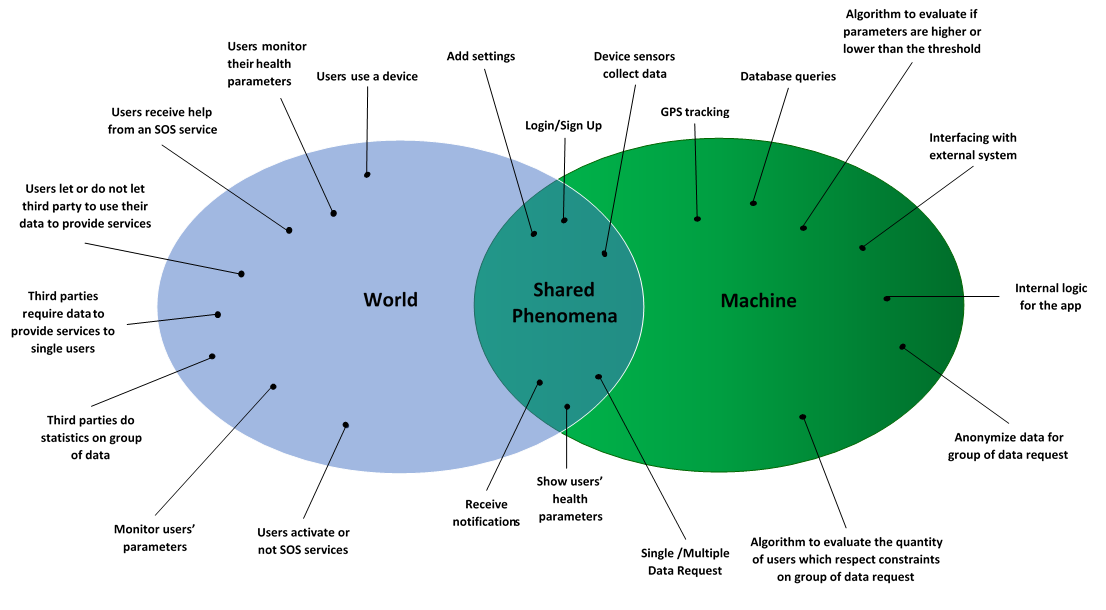
\includegraphics[width=1.00\textwidth]{./pictures/world_machine.png}\par
	\caption{Figure 1: World and Machine diagram}
\end{figure}

	\section{Definitions, Acronyms and Abbreviations}
	\subsection{Definitions}

\subsection{Acronyms}
	
\subsection{Abbreviations }
	\begin{itemize}
		\item {[Gn]: n-th goal}
		\item {[Dn]: n-th domain assumption}
		\item {[Rn]: n-th requiremnt}
	\end{itemize}




	\section{References}
	This document is strictly based on the specification concerning the DD assignment for the Software Engineering II project, part of the course held by professor Matteo Rossi and Elisabetta Di Nitto at the Politecnico di Milano, A.Y 2018/2019. It also refers to the RASD previously produced, more details about it can be found in the bibliography or in the GitHub repository.

	\section{Document Structure}
	This document consist in five sections:
\begin{itemize}
	\item \textbf{Section 1- Introduction:} In this chapter is given an overall view of the document, its goal and the informations to understand it's contents.
	\item \textbf{Section 2 - Architectural Design:} 
	\item \textbf{Section 3 - User Interface Design:} 
	\item \textbf{Section 4 - Requirements Traceability:}
	\item \textbf{Section 5 - Implementation, Integration and Test Plan:}
	\item \textbf{Appendix A:} contains the software and tools used, the bibliography and all efforts spent by each group component. 
\end{itemize}

	%Architectural design
	\chapter{Architectural Design}
	\label{ch: Architectural Design}

	\section{Overview}
	This section gives a detailed view of the physical and logical infrastructure

\subsection{High level component}
The app has been designed by applying the three layers architecture; this pattern, also kown as the n-tier architecture, is the de facto standard for most Java EE applications and devide in a well defined way the application's parts  by assigning a specific role to each layer.
\begin{itemize}
	\item \textbf{Presentation Layer:} It is the front end layer, it consists in the external interfaces and it is composed by three 			sublayers: two mobile application  dedicated to mobile devices, one for users and one for third parties, and a web browser for 			third parties.\\ Both mobile apps  includes only the presentation login and all sublayers directely interface with the app layer.
	\item \textbf{Application Layer:} It encases the app's core capability, this means that containts the whole logic included the main 		algorithms. 
	\item \textbf{Data Layer:} It includes the data storage system and data access. Data are accessed by the application layer 			via API call.
\end{itemize}In the following Figure the external services have been included to underline the fact that they interface with both presentation and application tier and it also underlines the fact that layers are closed. A closed layer means that a request moves from layer to layer and it  must pass through all layers right below before reaching the destination one.

\begin{figure}[h!]
	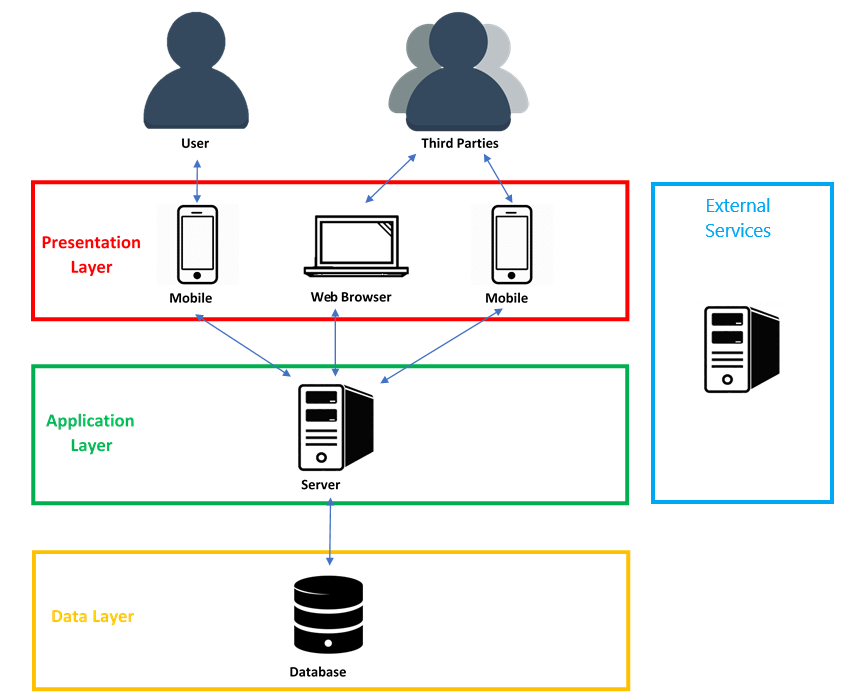
\includegraphics[width=1.0\textwidth]{./pictures/design_arch.png}\par
	\caption{Three-tiers architecture}
\end{figure}
\FloatBarrier

The next diagram shows interactions between all main components of the system. Because of the presence of two different stakeholders with different needs the client has been splitted in two according to the division in 2 different apps explained in the RASD. Althought this client's division the server has been maintained unique to avoid possible code redundancy and because most of the logic is related to the Third Party's app.

\begin{figure}[h!]
	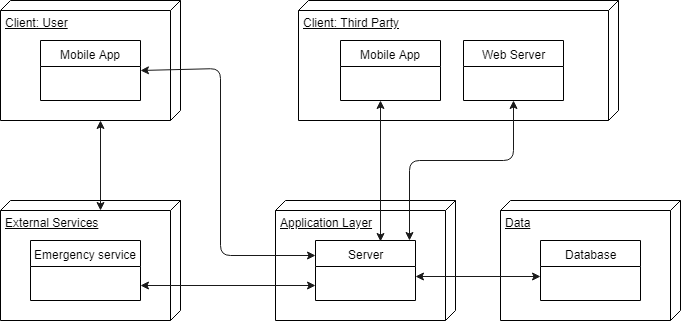
\includegraphics[width=1.0\textwidth]{./pictures/high_level_diagram.png}\par
	\caption{High Level Components}
\end{figure}
\FloatBarrier

	\section{Component View}
	\subsection{Components' Structure}
The presented Component Diagram has the aim to show in a more precise and detailed way which components are in each layer and how they interact.\\
To be more precise in the left it is possible to see the presentation layer devided in three components:
\begin{itemize}
	\item \textbf {User's Mobile App:} it is the user's application via device; that is the only possible interface for a user and it is 			formed by a \textit {Data Collector} and a \textit {Data Processor} components which have the aim to collect data from the 			external device containing all the necessary sensors to gather health parameters of every user ; a \textit {GPS Manager} 			which interfaces directly with the device's GPS needed in case of health parameter under the threshold (see RASD for 				more details); a \textit {GUI Manager} which is foundational to handle all actions made by users and a \textit {Controller} 			which is the bridge between the client's components and the application layer.
	\item \textbf {Third party's Mobile App:} it is the third party's application via device. This particular stakeholder doesn't need 			any GPS or Data manager because the aim of its app is to obtain data  of a single user or of a group of users, that's the 			reason why it is just formed by a \textit{ GUI Manager} and a \textit {Controller}. The aim of those two elements is the same 			presented for the user's mobile app.
	\item \textbf {Third Party's Web App:} the different aim of the app related to this stakeholder implies the necessity of a 			desktop application which is dial by the same components of the Mobile one.
\end{itemize}The application layer is also formed by three different components:
\begin{itemize}
	\item \textbf{Application Logic:} it contains the whole logic and algorithms which stay under the application and make it runs in 			a proper way. This component will be better analyzed in a dedicayìted subsection in which all its services will be presented into 			a class diagram. 
	\item \textbf{ ASOS Manager:} this component is in charge of interfacing with the external emergency service in case the 			related algorithms finds out that the user is an unhealthy one.
	\item \textbf{Data Persistence Unit:} it has a constant connection to the data layer and it has the aim to handle all possible 			dynamic behaviors related to operations on data.
\end{itemize}
\begin{figure}[h!]
	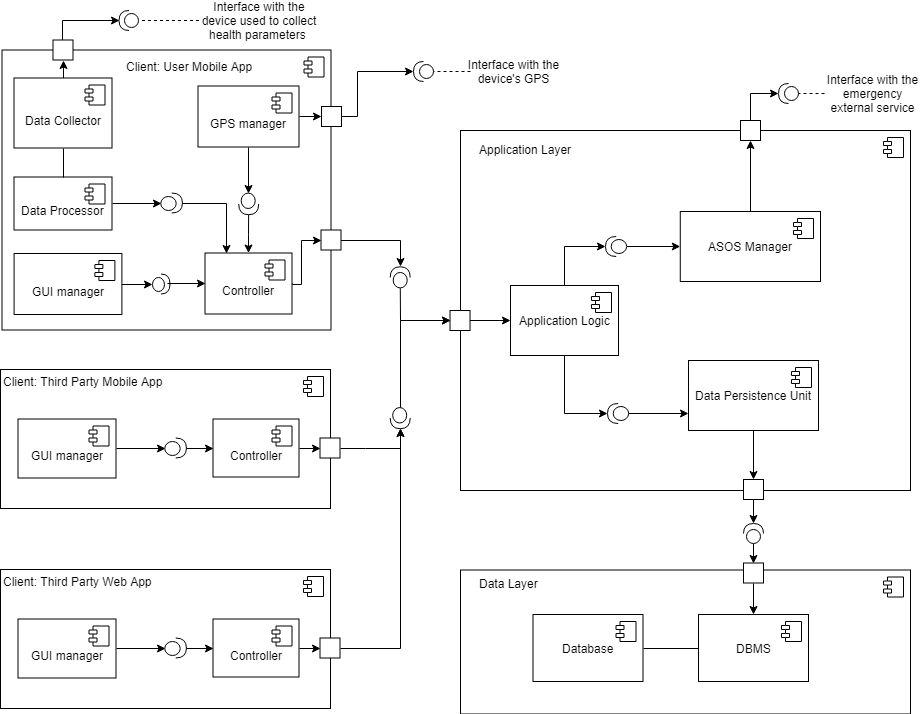
\includegraphics[width=1.0\textwidth]{./pictures/component_diagram.png}\par
	\caption{Component diagram}
\end{figure}
\FloatBarrier

\subsection{Application Logic}
To better describe the model's and controller's structure, is presented an UML class diagram more precise than the one in the RASD document. \\

\begin{figure}[h!]
	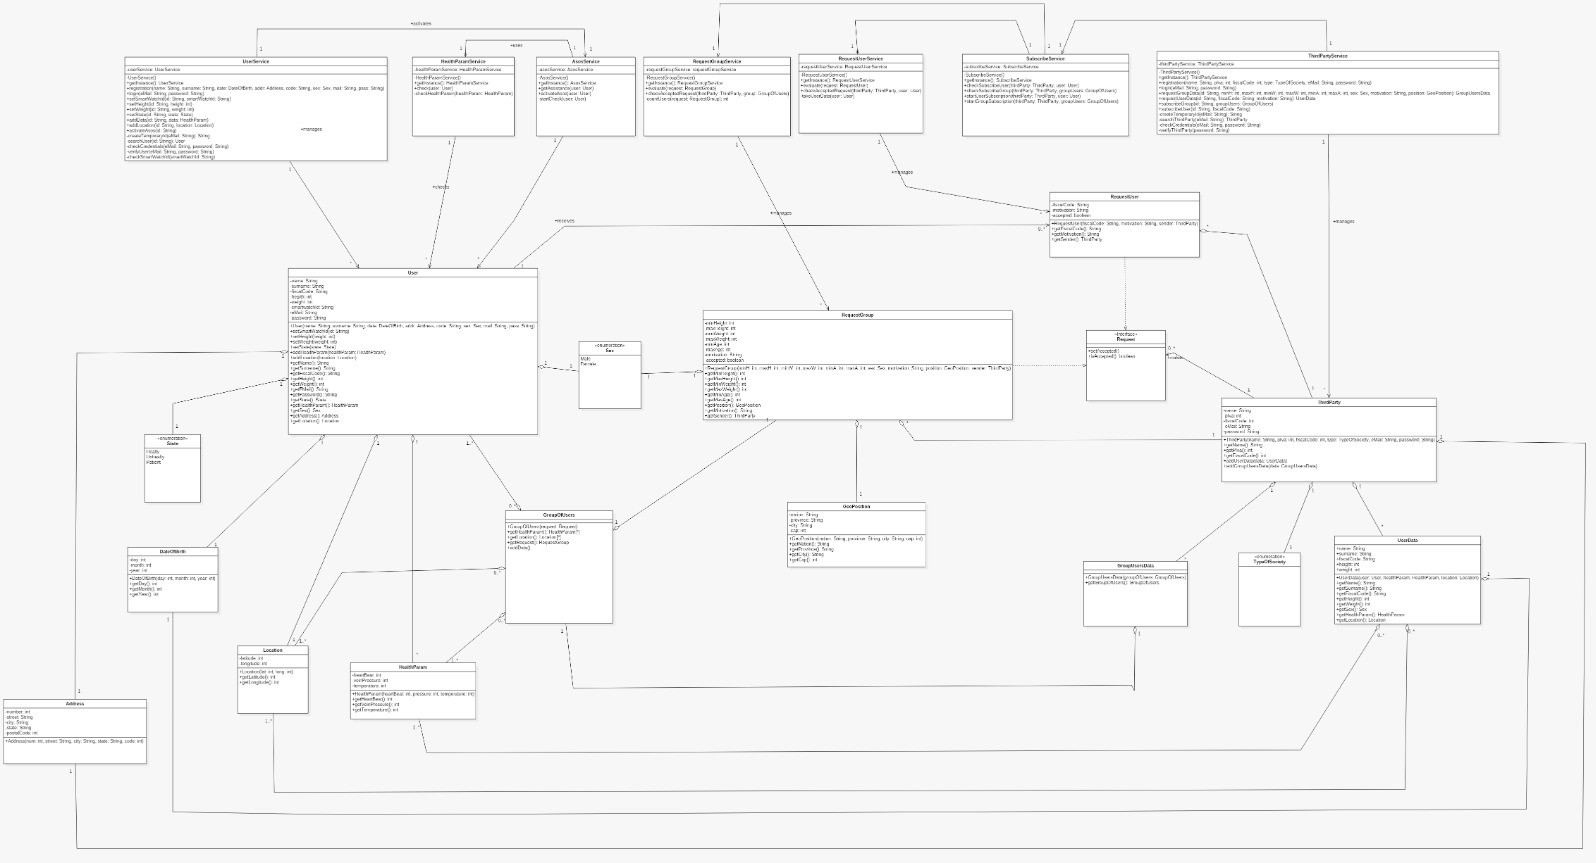
\includegraphics[width=1.0\textwidth]{./pictures/class_diagram.jpg}\par
	\caption{Class diagram showing the model of the appliation, it also contains all manager classes which have the aim to handle 			all possible dynamic actions.}
\end{figure}
\FloatBarrier
Note that the presented class diagram is intended as a guide for the implementation and integration of the model's part of the software.


\subsection{Database}
The data layer must contain the DB and also a DBMS component necessary to manage all possible operation, such as insertion, deletion, update, that can be done on data inside the storage unit. The chosen DBMS must guarantee the correct working of transaction according to the ACID properties.\\
A RDBMS is the best choice for this app because it adheres to the ACID properties; guarantees high performances by using indexis to sort data and by supporting both desktop and web apps and also guarantees data security providing a layer of protection for sensitive data. Using a RDBMS it is also possible to build  the DB structure and clearly define the relations between data.\\ 
As said in the previous section, the chosen architecture is composed by closed layers and for this reason  the data layer, the one which contains the stored data, can only be accessed by the Application's one, via a dedicated interface. Bacause of this it is necessary to provide a persistence unit which can handle all possible behaviors. Credentials and sensible data as personal informations must be encripted to avoid any possible privacy violation.\\
The Entity Relational diagram in figure describe a first relational model of the Database. The rectangual shapes represent the entities; the circles all possible attributes related to an entity in particular all cirles filled in black are the entities key and the relationships are represented by diamonds.

\begin{figure}[h!]
	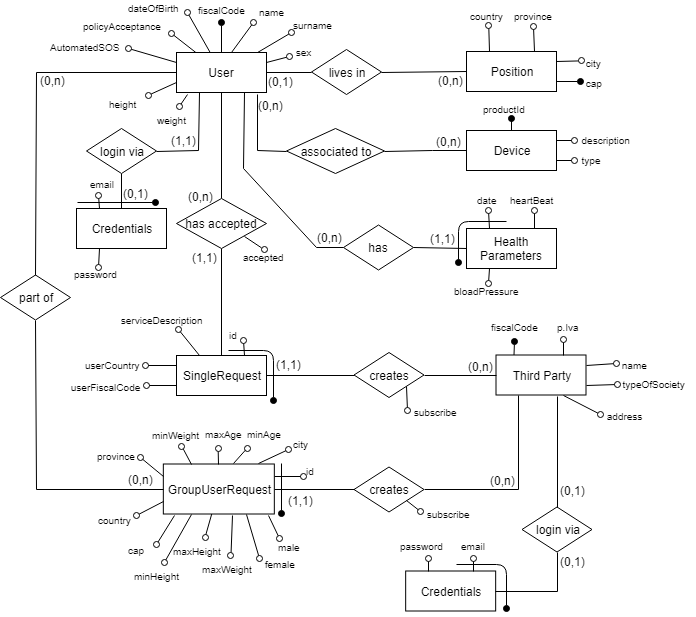
\includegraphics[width=1.0\textwidth]{./pictures/ER_diagram.png}\par
	\caption{Entity Relationship diagram}
\end{figure}
\FloatBarrier


	\section{Deployment view}
	\begin{figure}[h!]
	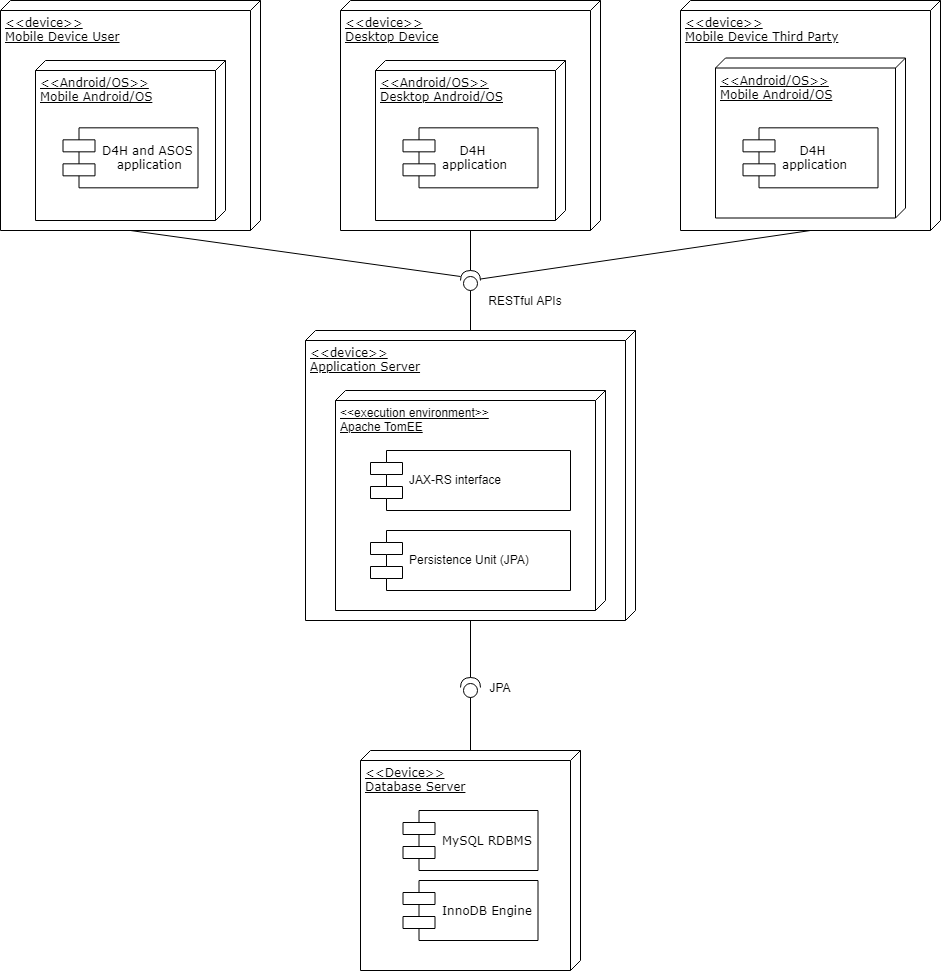
\includegraphics[width=1.0\textwidth]{./pictures/deployment_diagram.png}\par
	\caption{Deployment diagram}
\end{figure}
\FloatBarrier The Mobile App of users and third parties must be available on both IOS and Android systems; in order to obtain it the presentation layer must be code in Java for Android and in Swift for IOS.\\
In the diagram it is possible to find some implementation choices which are analyzed in the following lines.\\
It has been choice to use Java Enterprise Edition 8.2 (JEE) for the app layer because the aim of the final product is to become a large scope application with a great number of simultaneous clients and because, thanks to the ammount of APIs and tools the developers can focus on the main logic.
Here there are some choices made for the App Server implementation:
\begin{itemize}
	\item GlassFish or Jboss % still have to choose
	\item The RESTful APIs architecture is applied because it makes the efficiet use of the bandwidth and uses standard HTTP. It 			also has a great scalability and it allows to carry out basic operations;
	\item JAX-RS to implement proper REStful APIs to interface with clients;
	\item Java Persistence API (JPA) as persistence Unit to acces the database. It has been picked out because it is an Object/			Relational Mapping (ORM) framework applicable to RDBMS without implement direct SQL queries and because of its high 				performances , scalability, stability and quality.
\end{itemize}
The DB's implementation choices are the following:
\begin{itemize}
	\item JPA within the App Server as the interface to the DB;
	\item MySQL as the RDBMS;
	\item InnoDB as the data engine; this is already the default engine applied to every table generated in MySQL but it has been 			choice because it associates high performances to high data consictency and integrity. To let this happens, this particular 			engine has developed some particular functionalities such as the introduction of foreign keys; locks at row level; MVCC to 			increment the concurrency in queries and support in tansactions to guarantee correctness in data.
\end{itemize}

\begin{figure}[h!]
	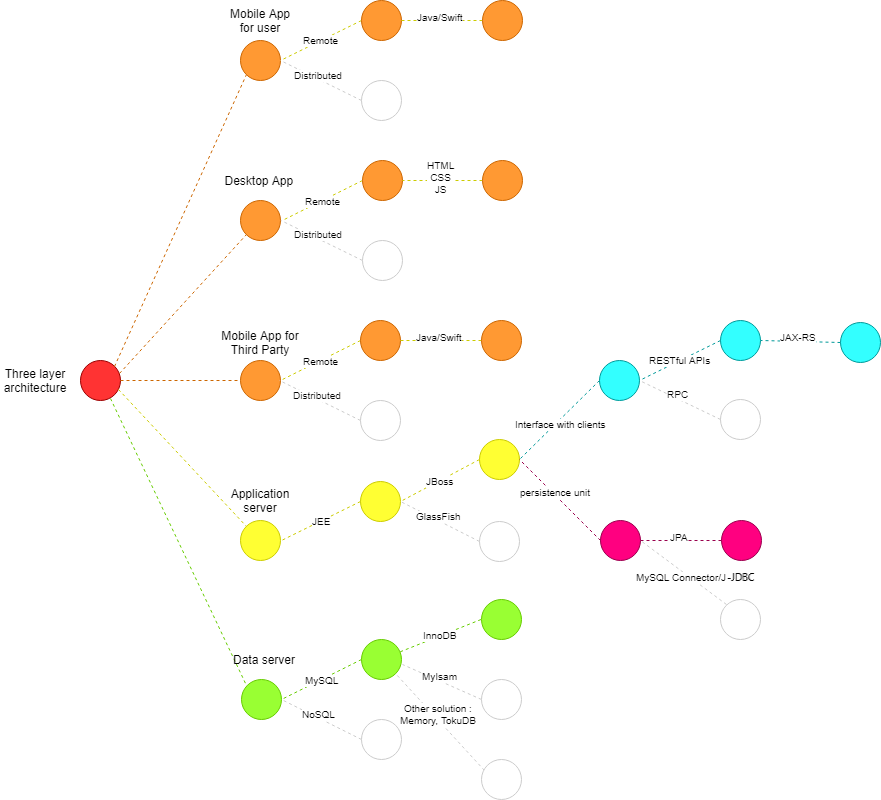
\includegraphics[width=0.80\textwidth]{./pictures/choice_diagram.png}\par
	\caption{The aim of this figure is to show which implementation possibilities have been discarded.It represents the decision 			tree for the starting architectural design. }
\end{figure}
\FloatBarrier


	\section{Runtime view}
	The runtime view of the software is described by a set of UML sequence diagrams that shows how the software will behave.\\
Note that the processes of registration and login are analyzed only for users but they are very similar for third parties.

\begin{figure}[h!]
	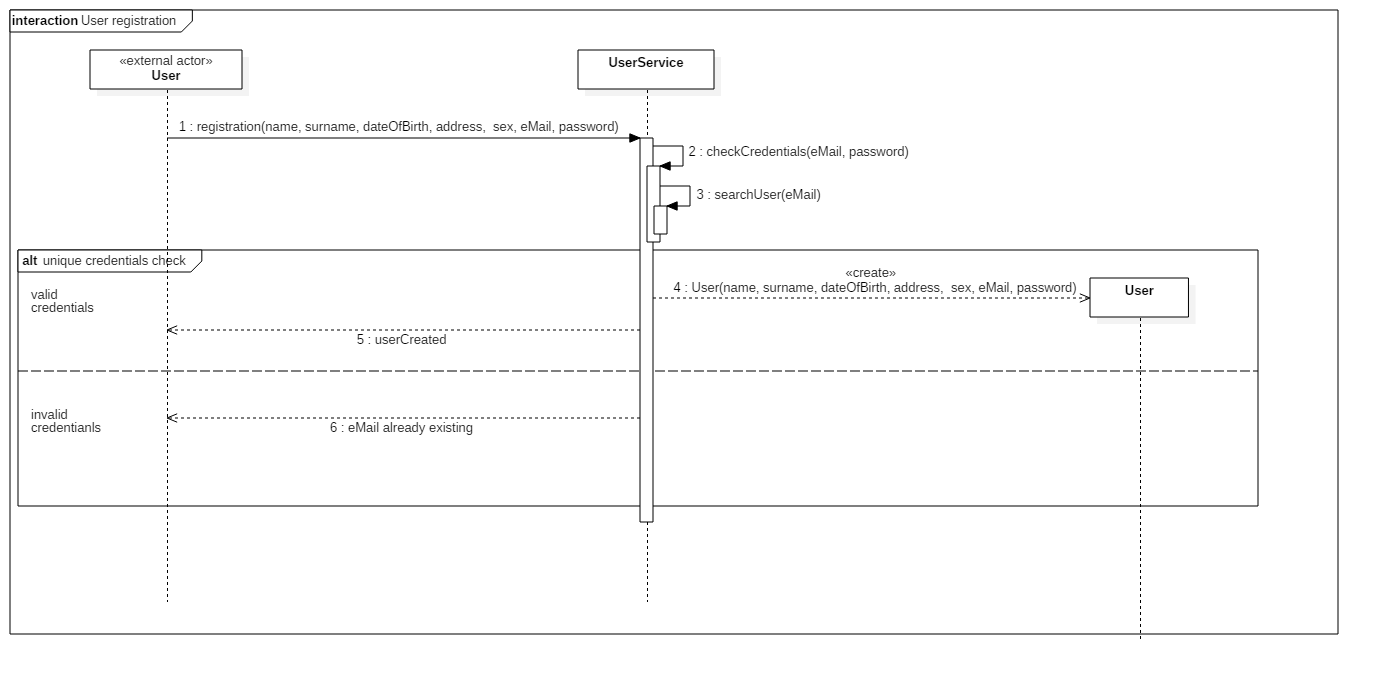
\includegraphics[width=1.0\textwidth]{./pictures/sequence_userRegistration.png}\par
	\caption{Sequence diagram about the registration of a user.}
\end{figure}
\FloatBarrier 

\begin{figure}[h!]
	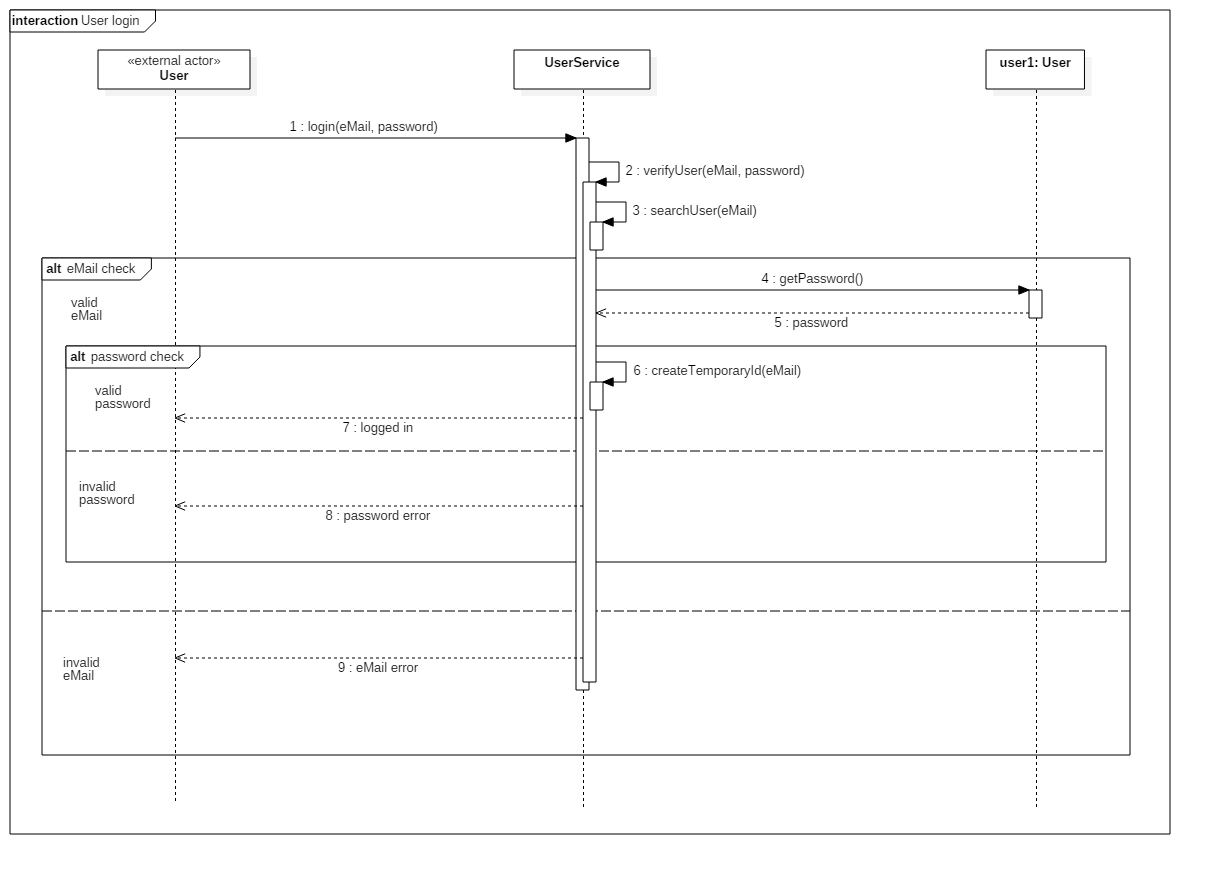
\includegraphics[width=1.0\textwidth]{./pictures/sequence_userLogin.png}\par
	\caption{Sequence diagram about the login of a user.}
\end{figure}
\FloatBarrier 

\begin{figure}[h!]
	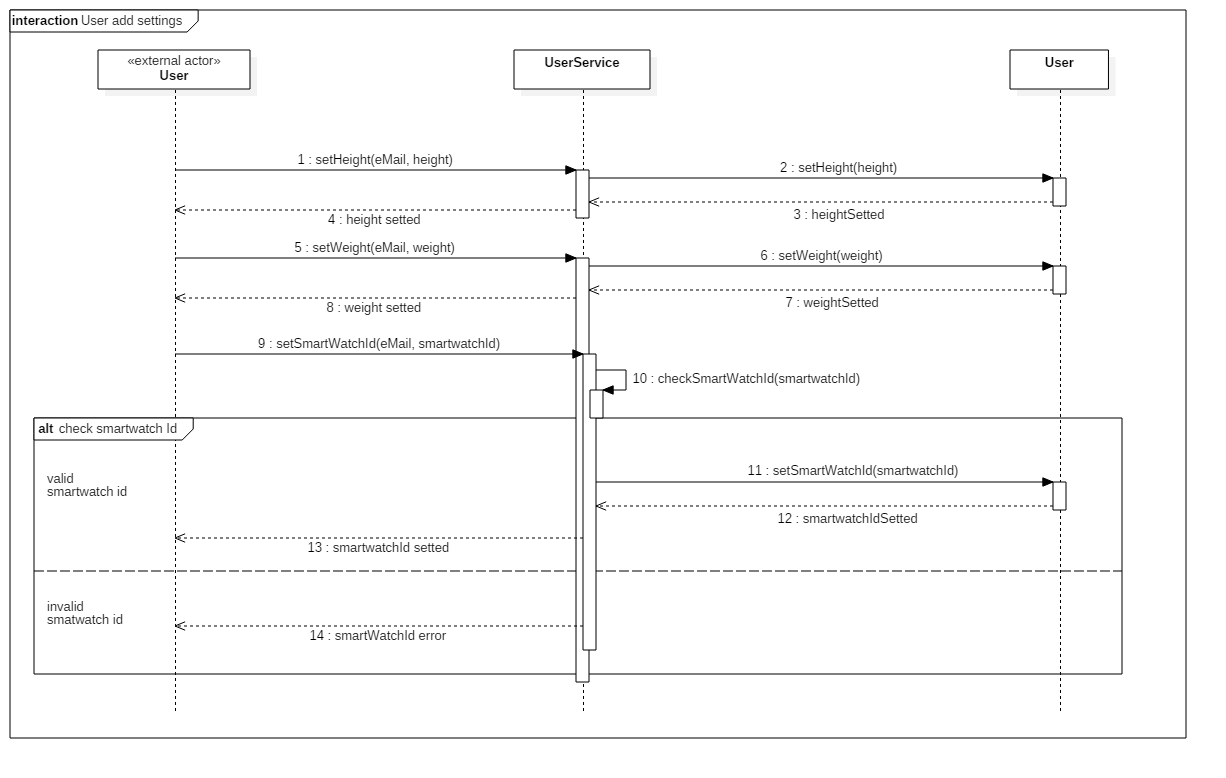
\includegraphics[width=1.0\textwidth]{./pictures/sequence_userSettings.png}\par
	\caption{Sequence diagram about adding a user's settings.}
\end{figure}
\FloatBarrier 

\begin{figure}[h!]
	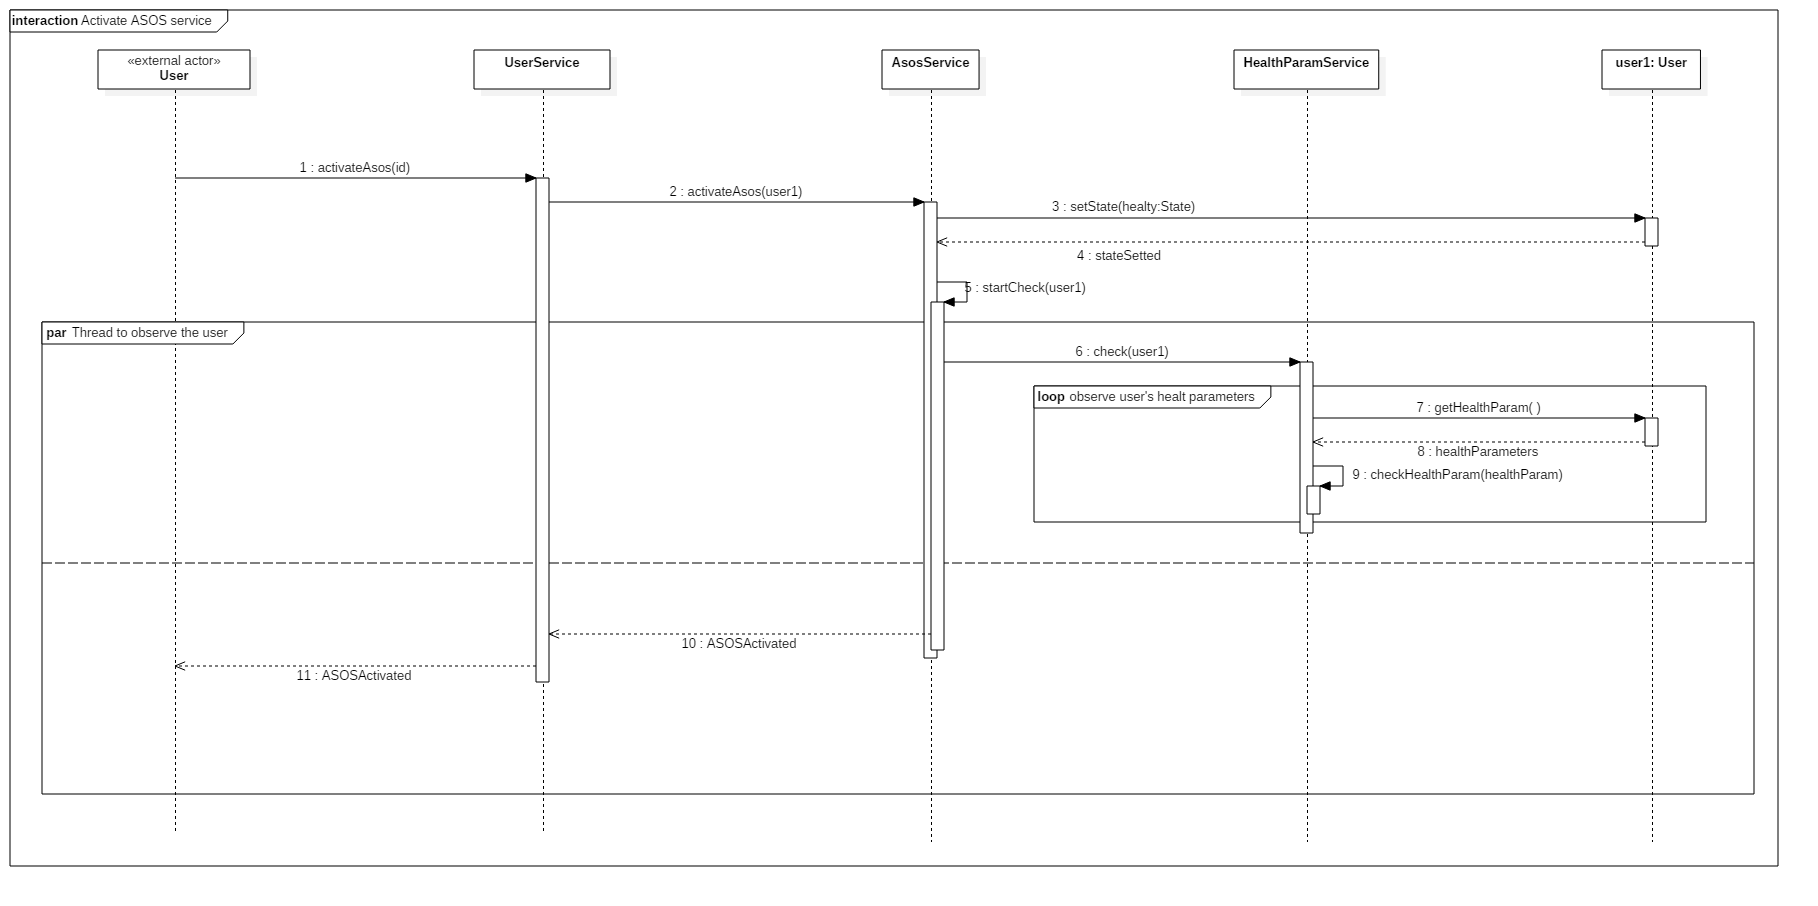
\includegraphics[width=1.0\textwidth]{./pictures/sequence_activateAsos.png}\par
	\caption{Sequence diagram about the activation of ASOS.}
\end{figure}
\FloatBarrier 

\begin{figure}[h!]
	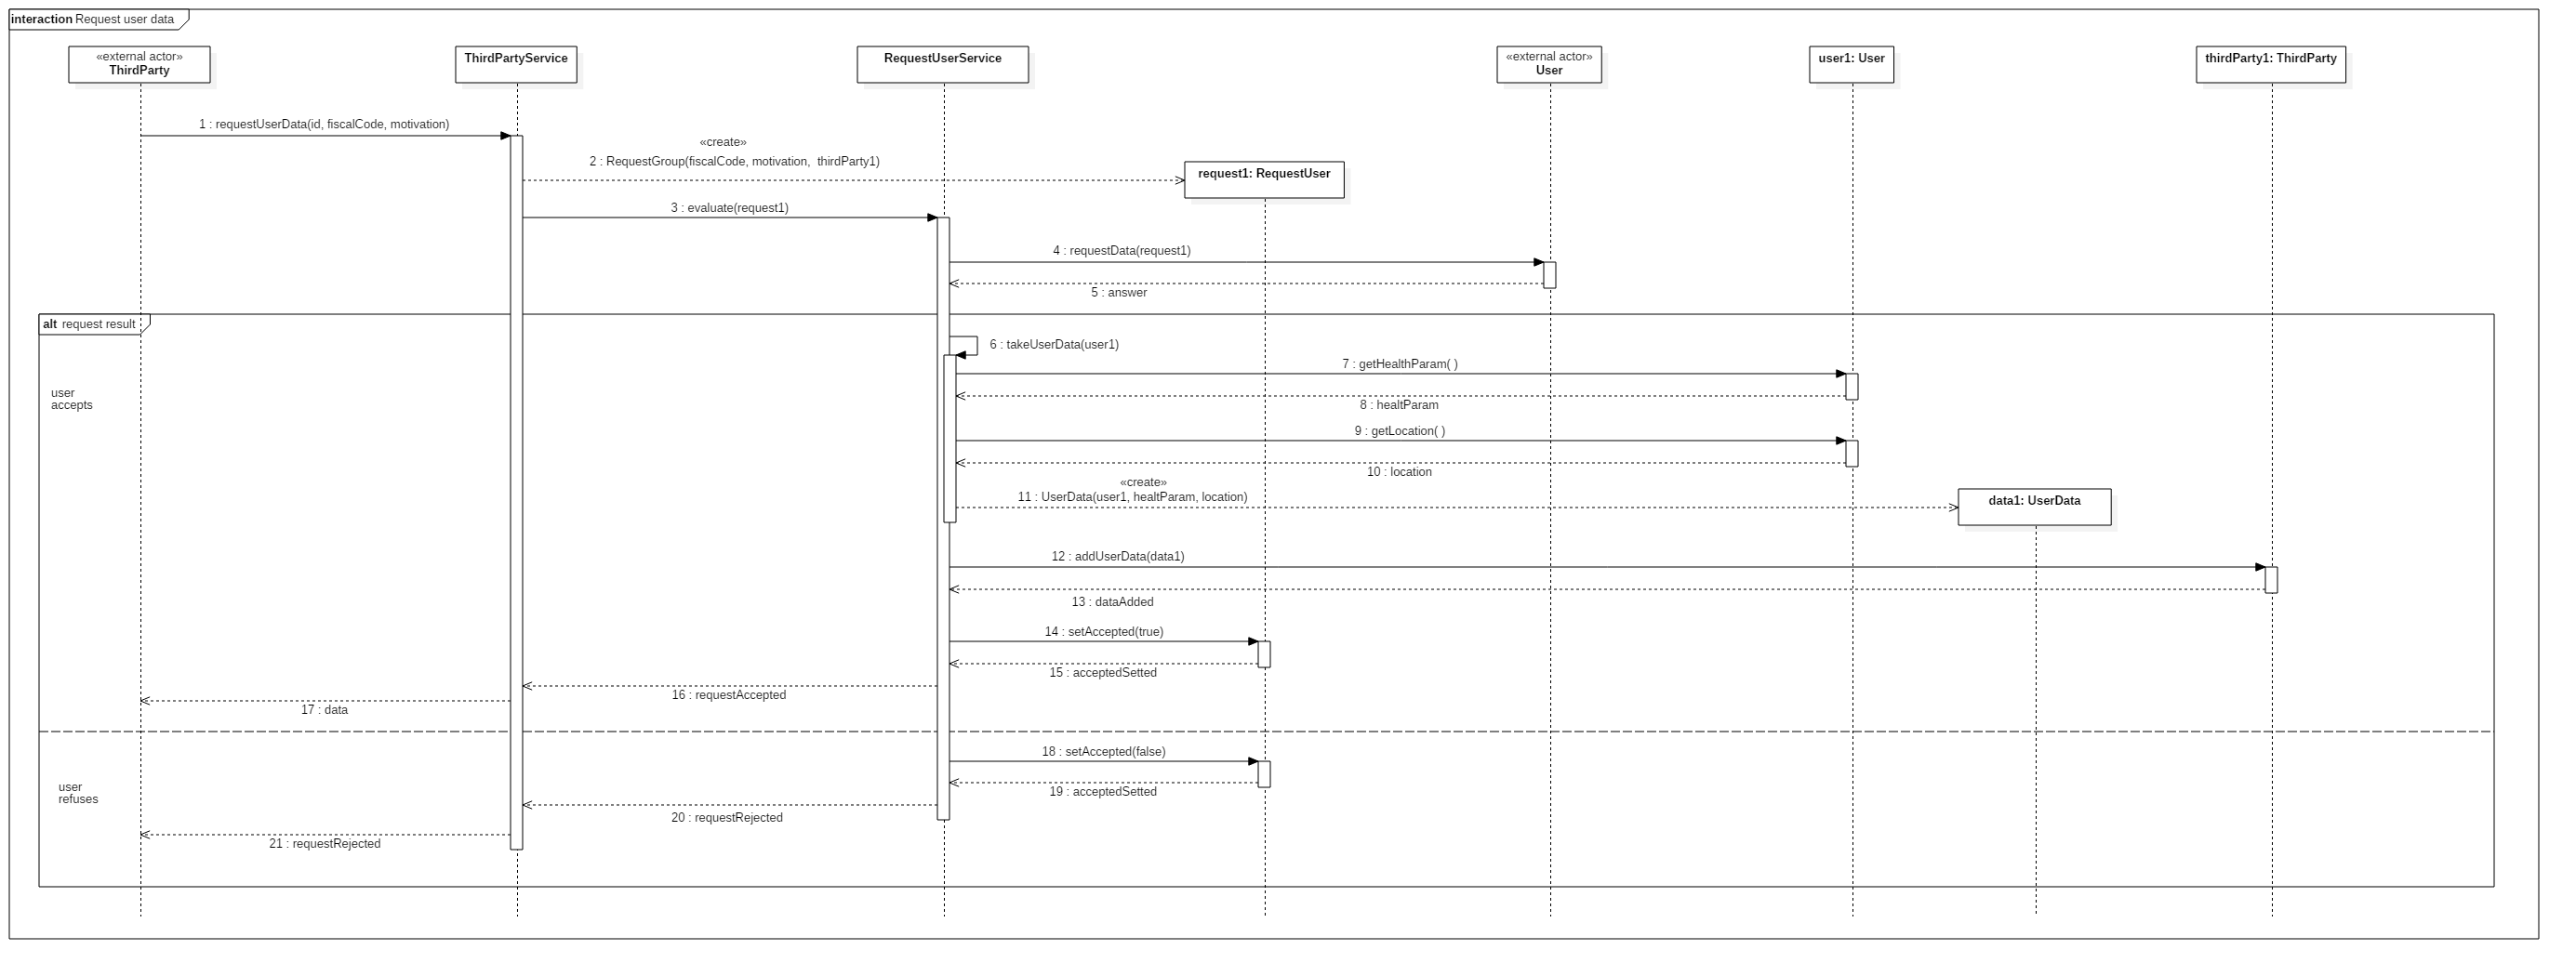
\includegraphics[width=1.0\textwidth]{./pictures/sequence_userRequest.png}\par
	\caption{Sequence diagram about requesting data about a user.}
\end{figure}
\FloatBarrier 

\begin{figure}[h!]
	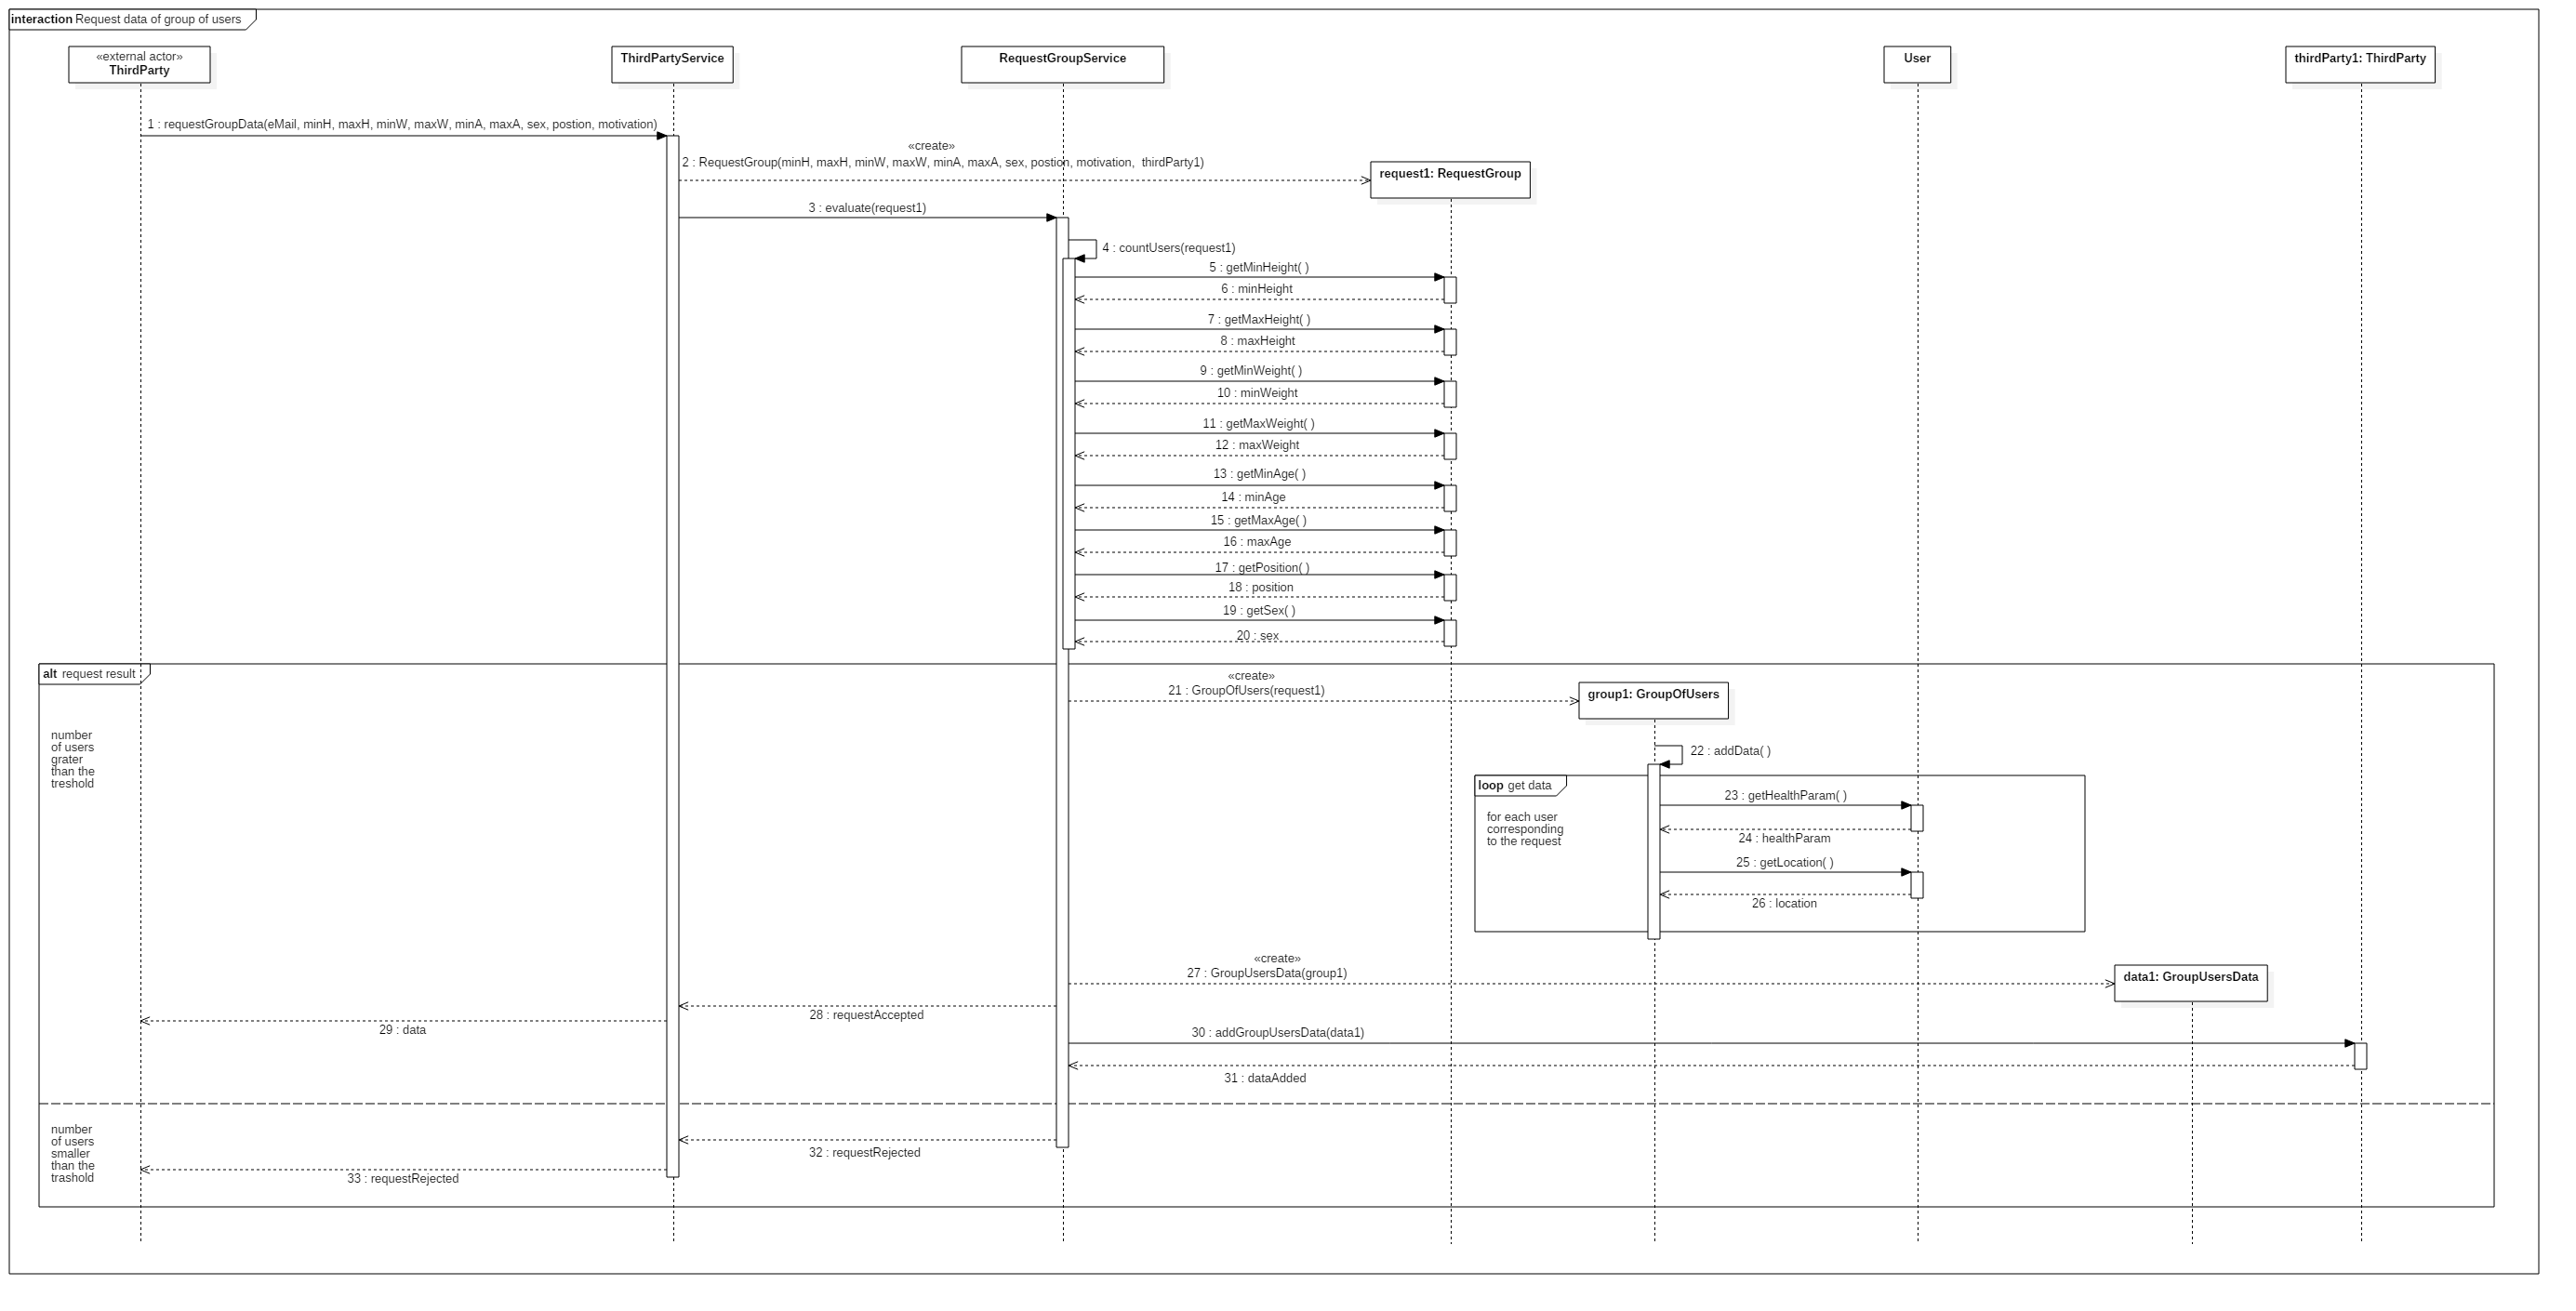
\includegraphics[width=1.0\textwidth]{./pictures/sequence_groupRequest.png}\par
	\caption{Sequence diagram about requesting data about a group of users.}
\end{figure}
\FloatBarrier 

\begin{figure}[h!]
	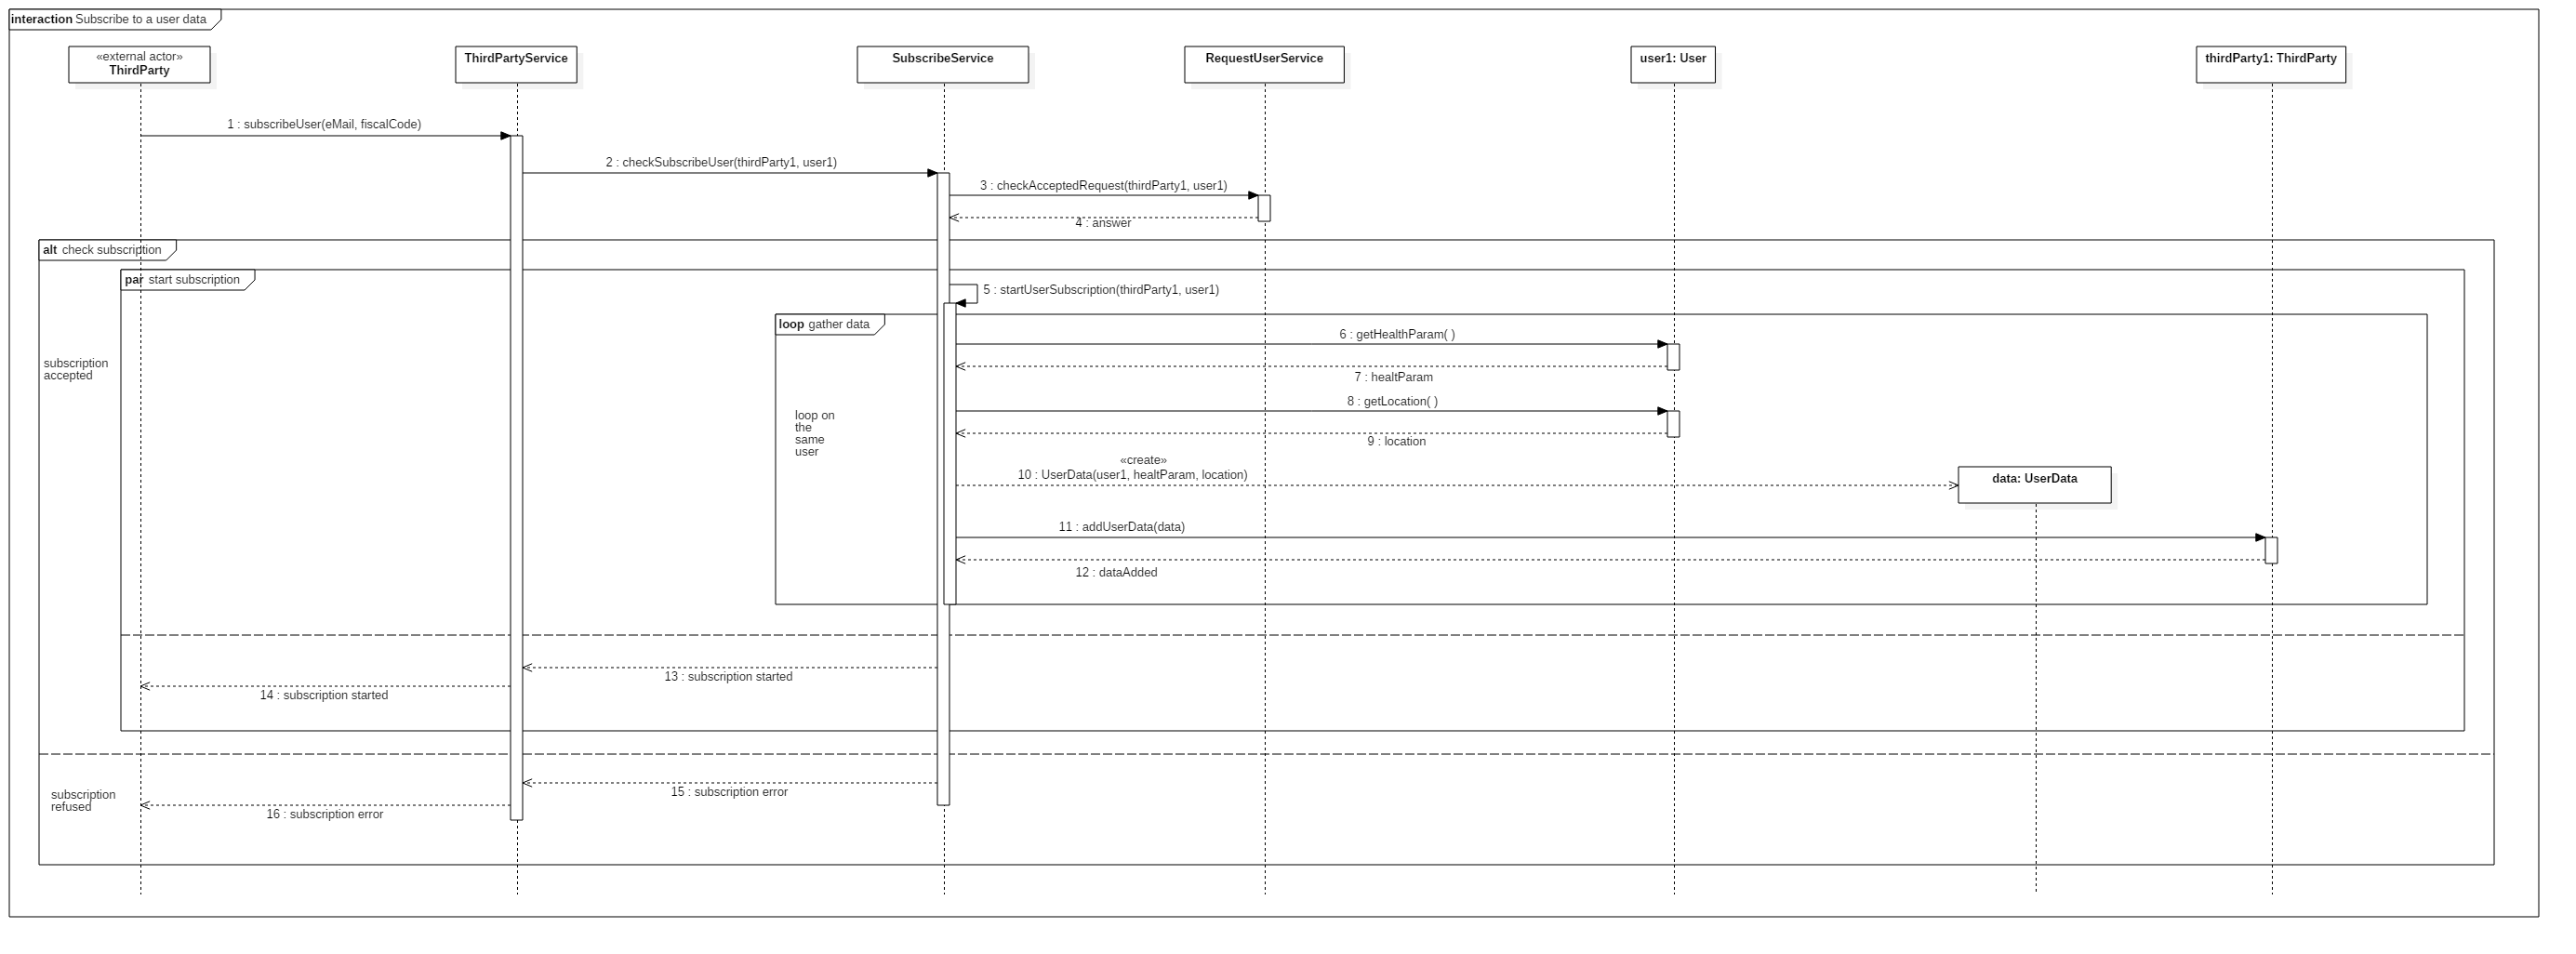
\includegraphics[width=1.0\textwidth]{./pictures/sequence_userSubscribe.png}\par
	\caption{Sequence diagram about subscribing to a user data.}
\end{figure}
\FloatBarrier 

\begin{figure}[h!]
	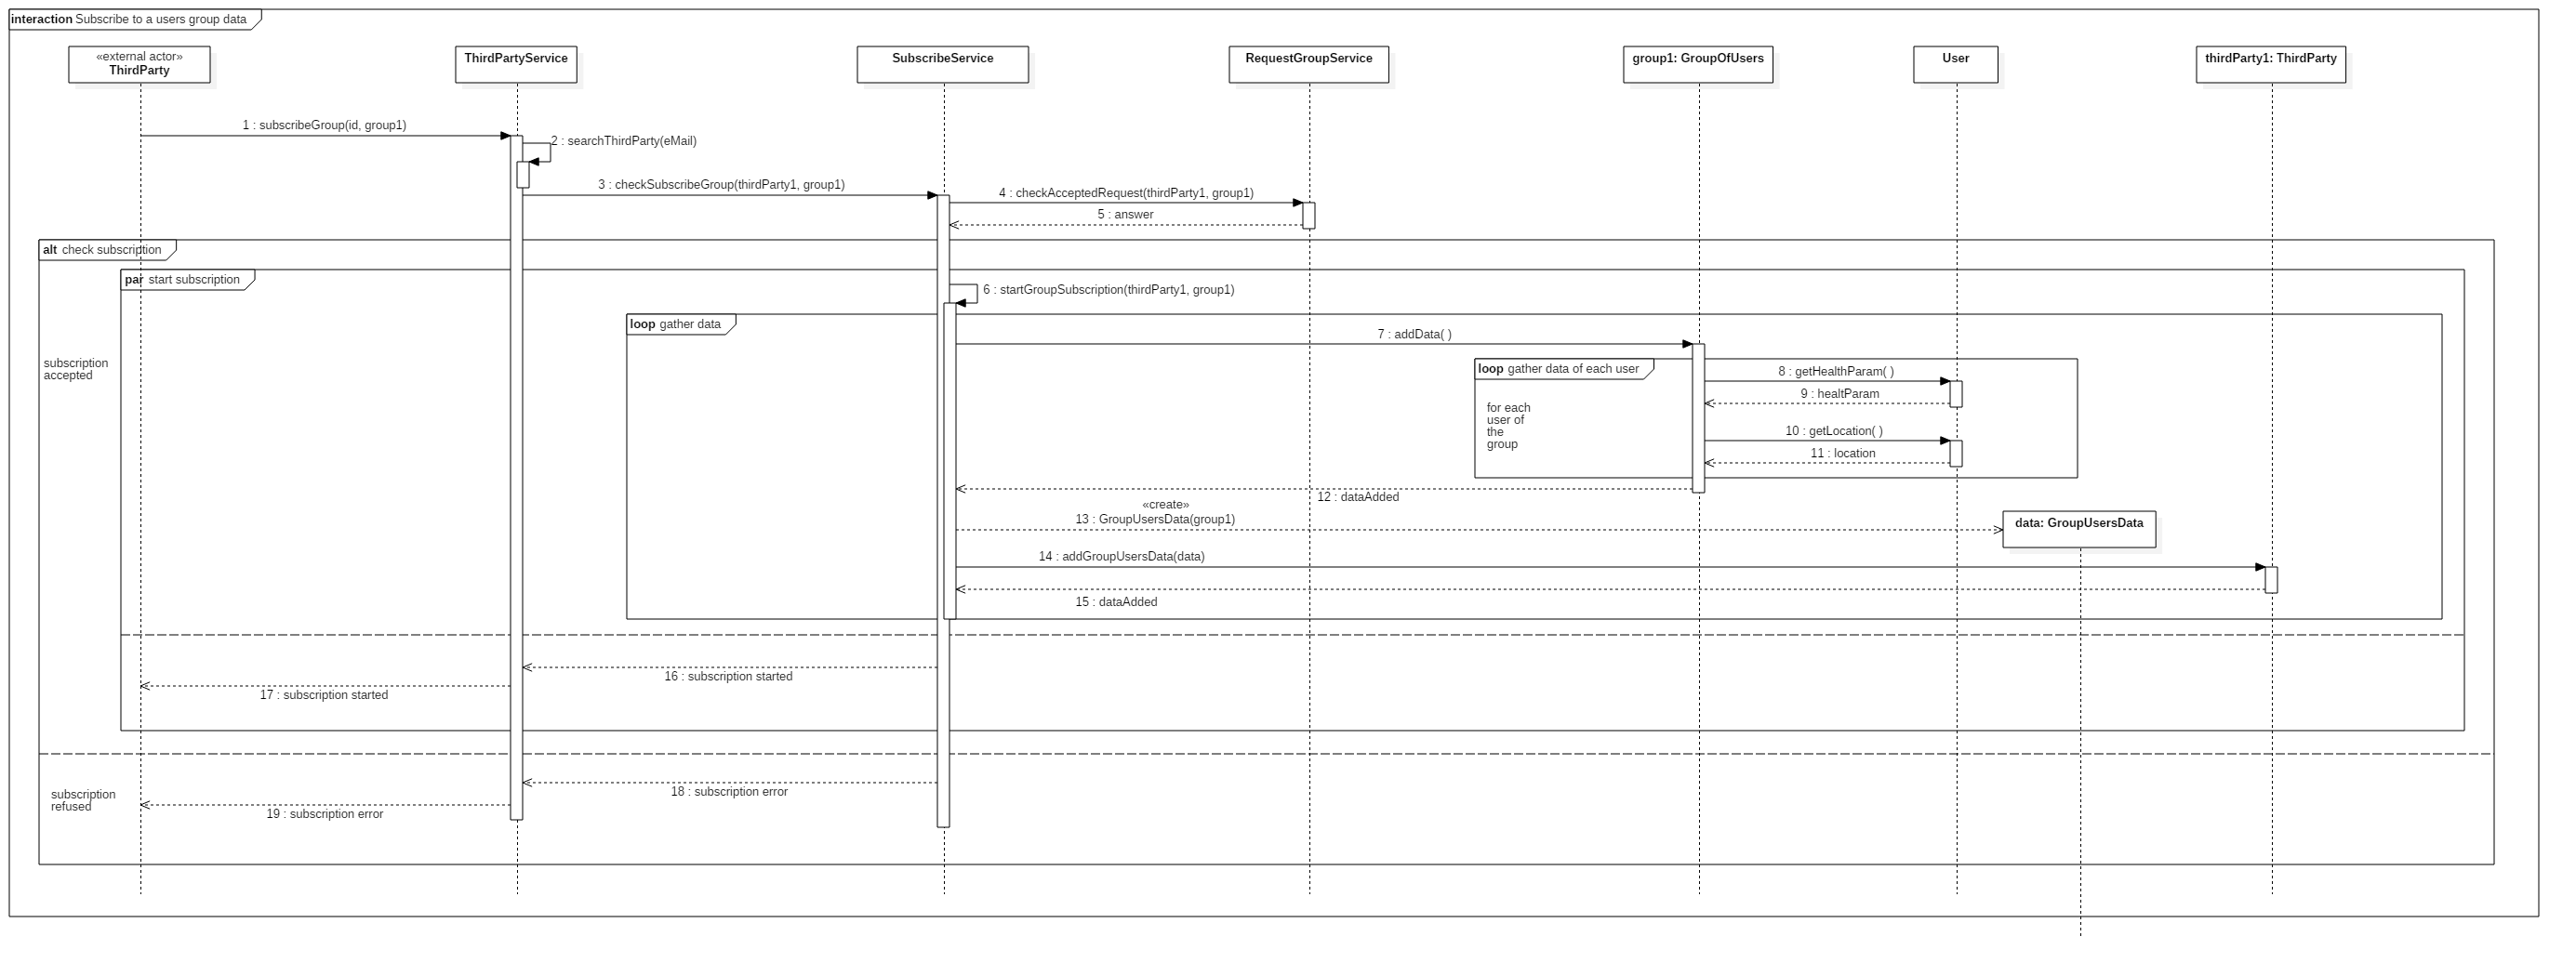
\includegraphics[width=1.0\textwidth]{./pictures/sequence_groupSubscribe.png}\par
	\caption{Sequence diagram about subscribing to a users group data.}
\end{figure}
\FloatBarrier 

\begin{figure}[h!]
	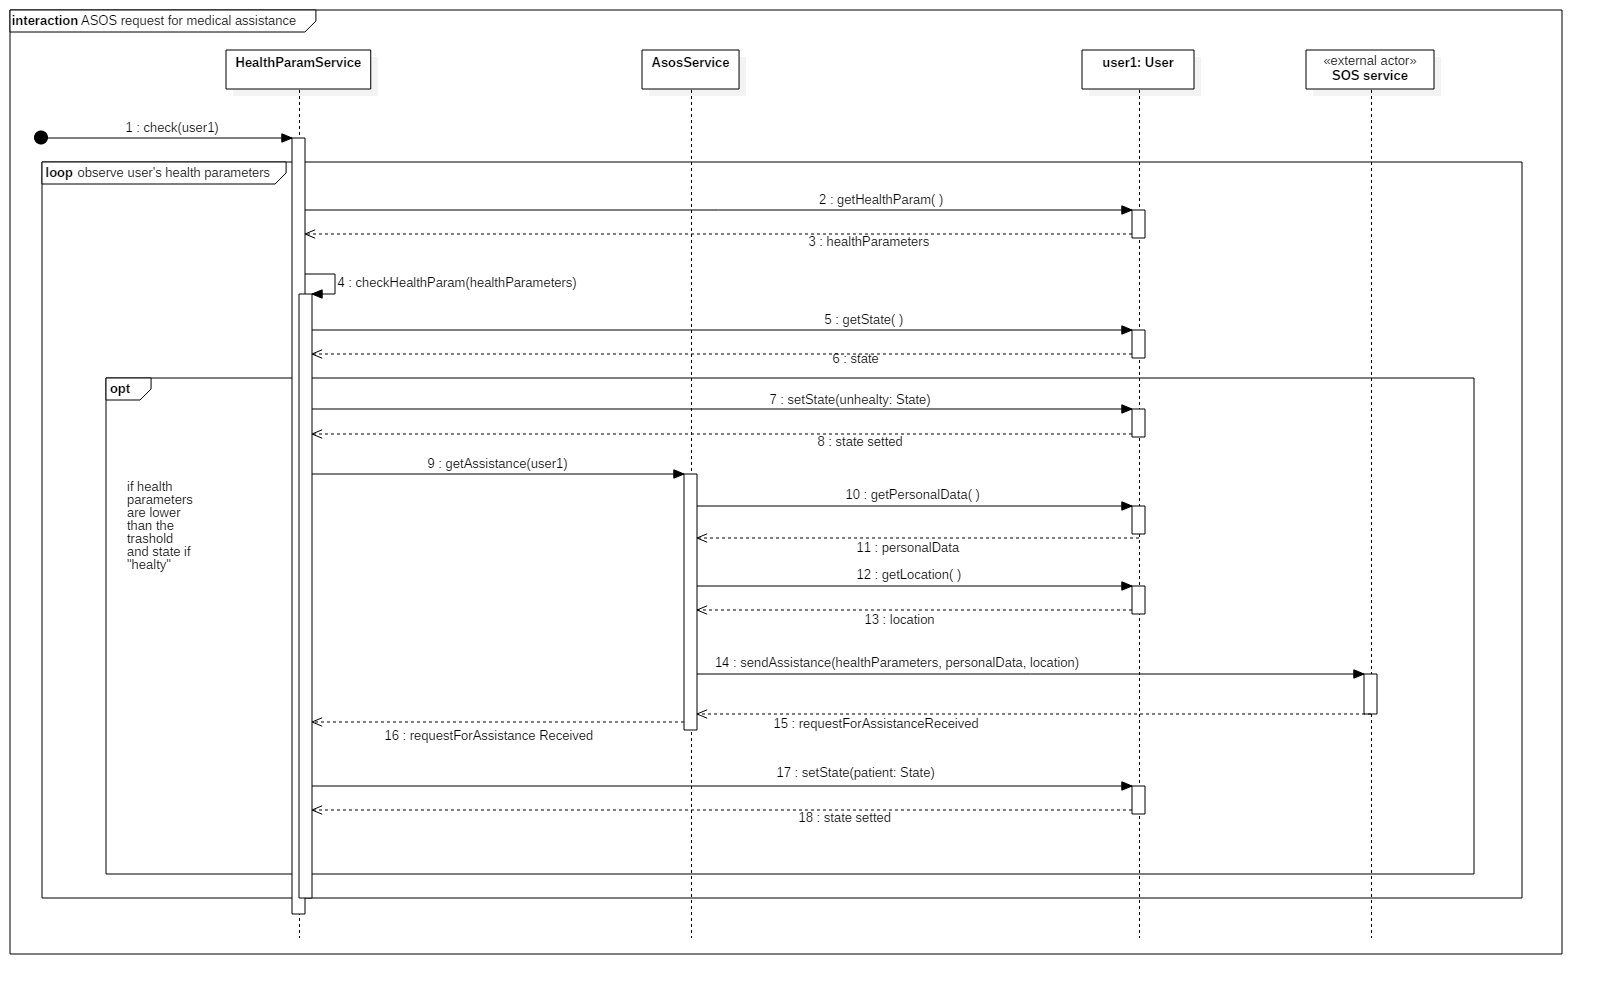
\includegraphics[width=1.0\textwidth]{./pictures/sequence_useAsos.png}\par
	\caption{Sequence diagram about ASOS requesting for assistance for a user.}
\end{figure}
\FloatBarrier 

	\section{Component Interfaces}

	\section{Selected architectural styles and patterns}
	The following styles and patterns have been used:

\subsubsection{Three layer architecture}
As already said in section 2.1 it has been chosen a three layer architecture formed by the Presentation layer, the Application layer and the Data layer. The use of this architecture allows to phisically divide presentation, application processing and data operations.\\
The presentation layer is extensive and includes both users and third parties interactions in various device (multichannel access) and tools for managing the tier. It is implemented based on the design pattern MVC (Model-View-Controller)  but the direct link to the data layer is connected to the app tier, which is made accessible using services components, consisting of the service model of the application.

\subsubsection{Thin Client for Third Parties}
It has been chosen to use the thin client approach while designing the interaction between third parties' devices and the system. Because of this the main logic is implemented by the App Server, which has been designed to have sufficient computing power and to work in an efficient way. It has also been picked because, by this way, the app via device doesn't take to much space, it can work even in case of limited computing power and it can be updated in an easier way.

\subsubsection{Thick Client for Users}
The thick client approach has been picked while designing the interaction between users' devices and the system. Even though the main logic is still implemented by the App Server, this type of client has been chosen to deal with the associated devices' sensors devoted to collect the user's health parameters. However, the added logic shouldn't require to much space, so also the users' application should still be lightweight and easily updatable.

\subsubsection{Model-View-Controller}
The system is design using the Model-View-Controller (MVC) pattern which separates internal representations of information from the ways information is presented to and accepted from the user. 
\begin{itemize}
	\item The model directly manages data, logic and rules of the application while beeing independent of the user interface.
	\item The controller receives all the users' inputs and performs their requests interacting with the model.
	\item The view gives a representation of the model to the users.
\end{itemize}
The choice of using the MVC pattern is made because goes well with the three layer architecture and garants efficient code reuse and parallel development.

\subsubsection{Singleton}
The model's "service" classes are designed as singletons. Those includes UserService and ThirdPartyService which are the classes in charge of manage the interactions with clients; RequestUserService and RequestGroupService which manages data requestes made by third parties; SubscribeService which gather data from users and group of users and gives them to third parties; HealthParamService and AsosService which are in charge of monitor health parameters of users and send assistance to them if their health parameters goes below a certain threshold. \\
The choice of design these classes as singletons is made because is needed only one object of them to coordinate actions across the system.


	\section{Other design decisions}
	\subsubsection{Password Security}
In order to guarantee the highest possible secutiry of credentials, they won't just be encripted but they will be also salted; this choice has been made because people usually reuse the same password and becasue it is the access key to the personal area and personal data which must be protect from strangers.

\subsubsection{Location}
To obtain the location in which the user is it is necessary a map service. Instead of develop a new map app, the Google Maps's service is the most reasonable choice bacuse it is already implemented and offers all needed services. It will be used to obtain the precise coordinates in which the user is, this is foundamental in case of an unhealty user bacause the location will be immediately transmit to the external emergency service via the ASOS manager.

	%User interface design
	\chapter{User Interface Design}
	\label{ch: User Interface Design}
	In this section there aren't mockups showing the design of the mobile apps because they have already been inserted in the RASD but there are mockups representing the third parties' desktop application.\\
After a reasonable analysis of the real world in which the final product will be insert, the third parties' app has been designed as a multichannel application . Third parties are companies, no profit societies, govarnement offices so it is reasonable to think that the main way to access to the app is via one or more desktops inside them; it has been chosen to add also the mobile version to obtain a larger possible base of third parties.\\
There are also two UI flowchart diagram representing the different screens provided by the apps and the dynamic contents. The purpose of these diagrams is to show the interaction among different scenes, which actions that let to moove from one scene to the other and which actions generate errors.\\
Even though there are three GUI, only two diagrams can be found in this section because the third parties's app is a multichannel one and both desktop and mobile app implements the same functinalities.\\
All images in the diagrams have been taken by the RASD,section 3.  
\section{UI diagrams}
\begin{figure}[h!]
	\centering
	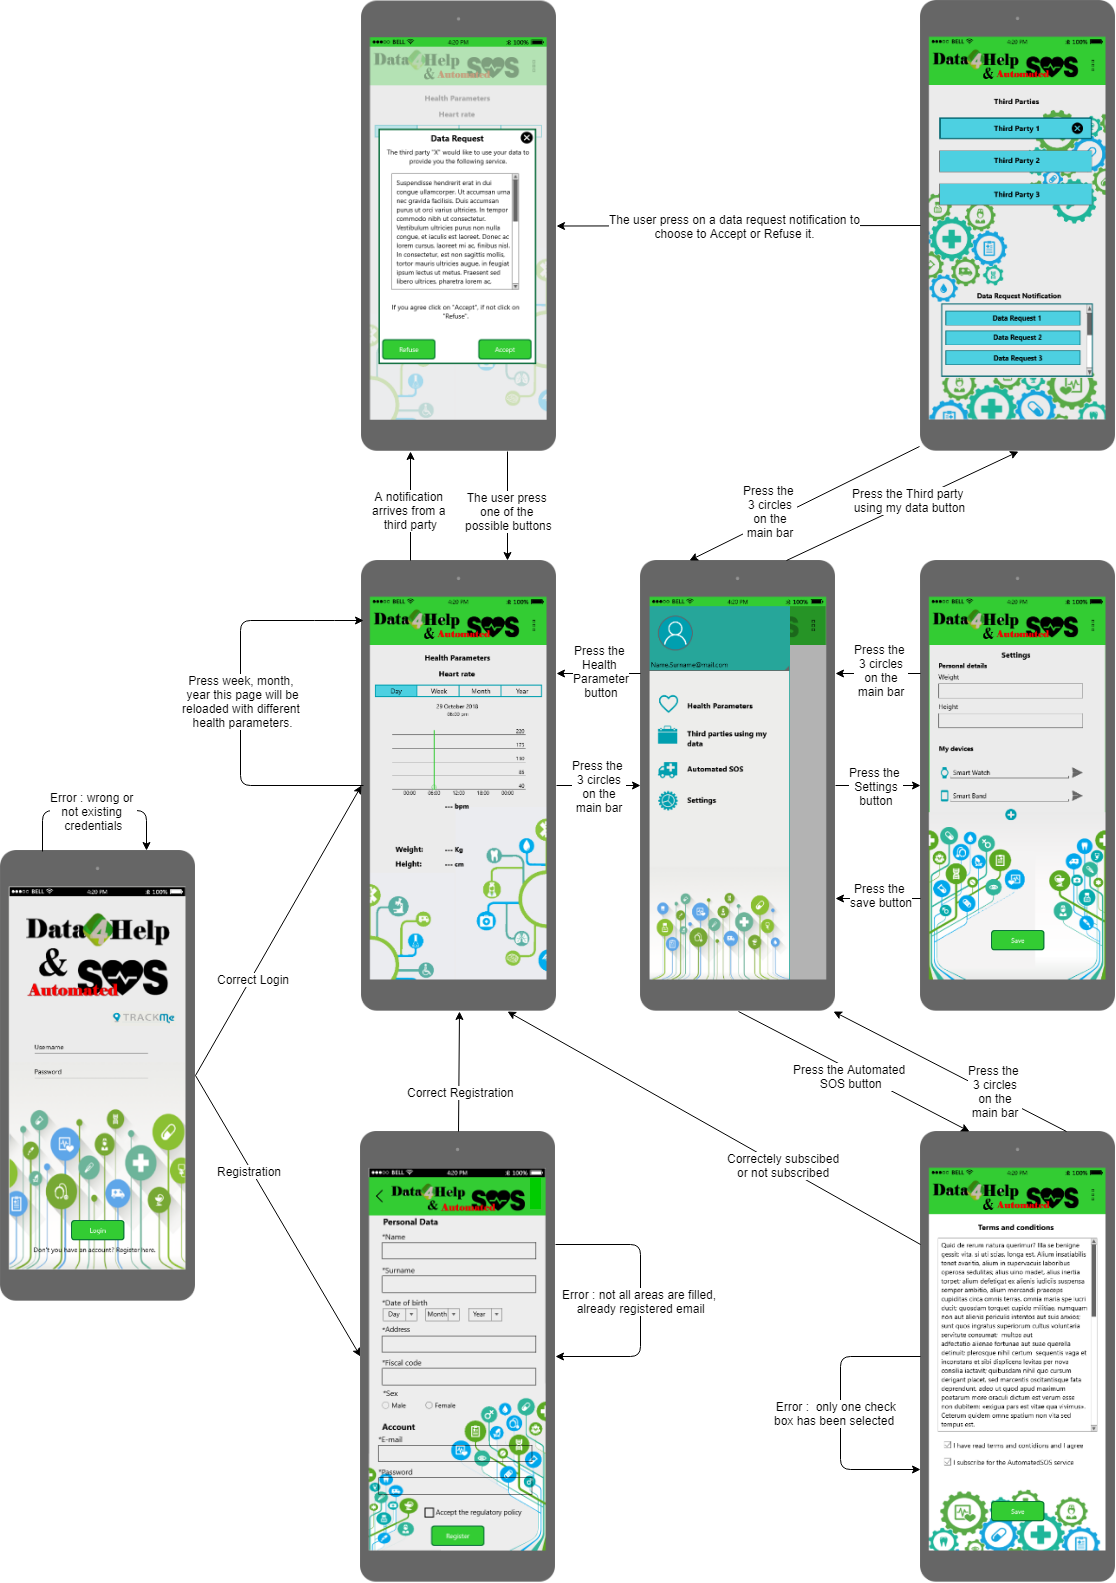
\includegraphics[width=1.0\textwidth]{./pictures/UI_flowchart_diagram.png}\par
	\caption{UI flowchart diagram of the users' mobile app.}
\end{figure}
\FloatBarrier
\begin{figure}[h!]
	\centering
	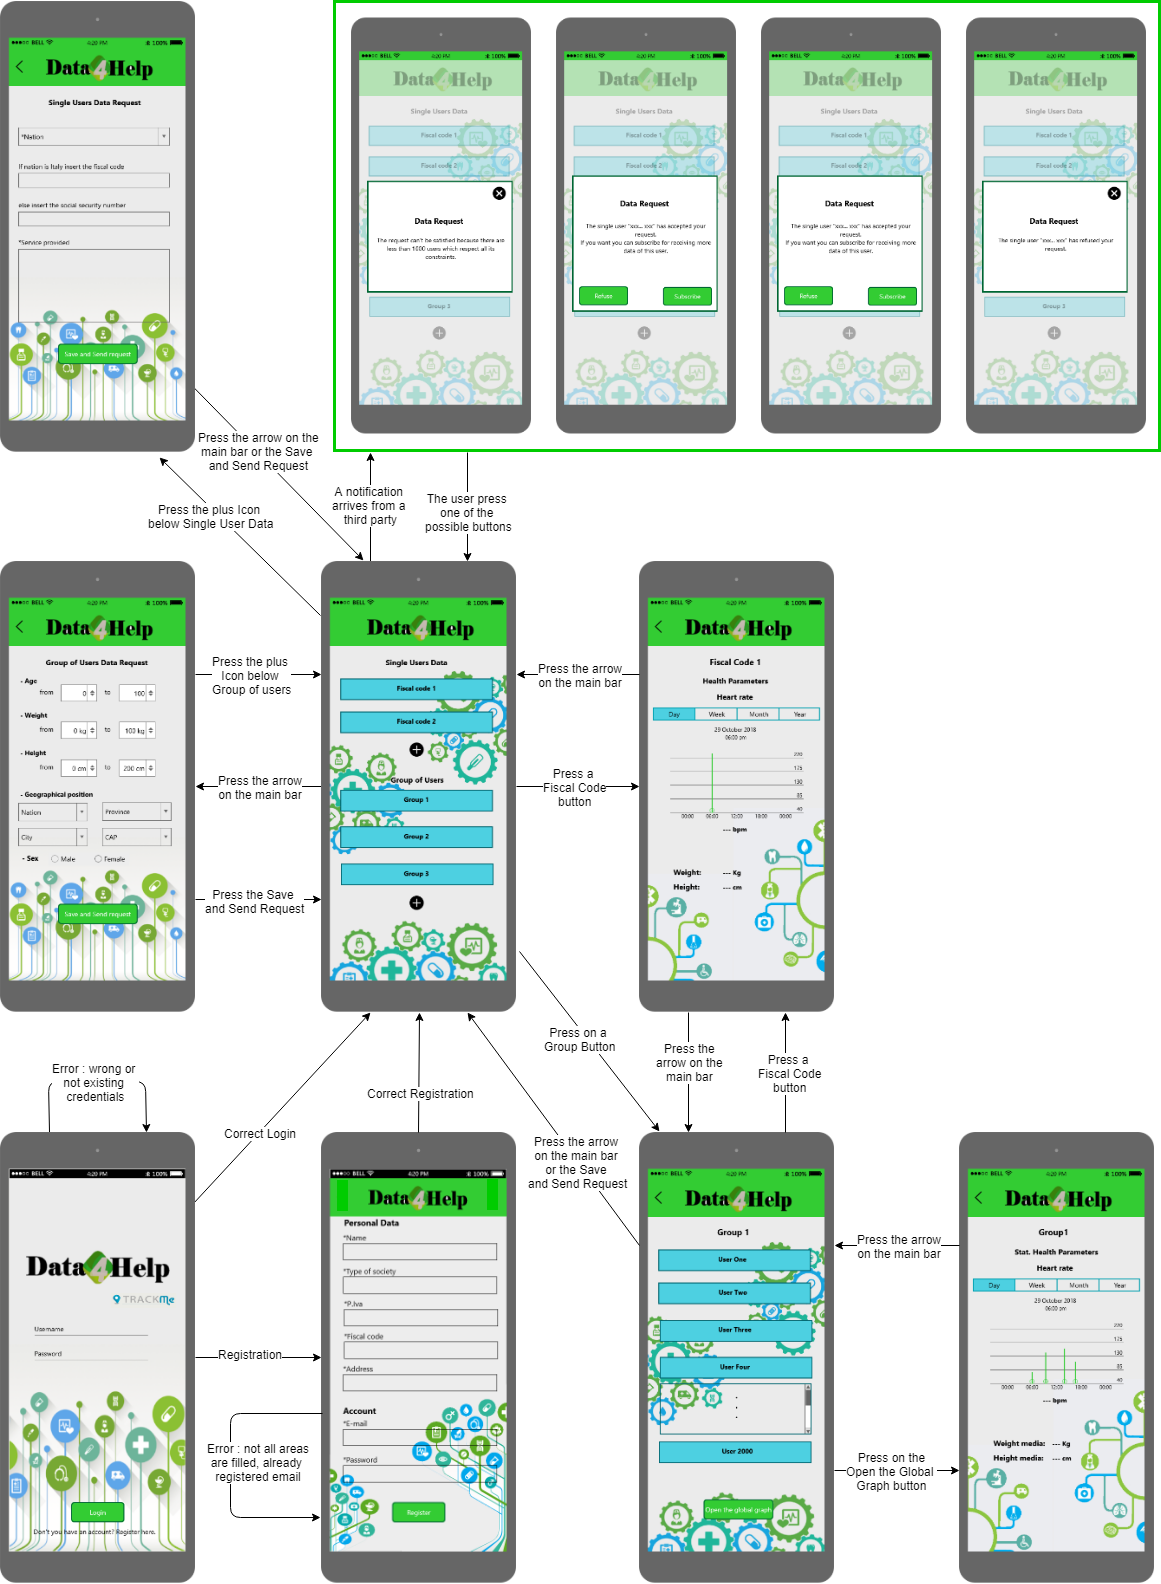
\includegraphics[width=0.90\textwidth]{./pictures/tp_UI_flowchart_diagram.png}\par
	\caption{UI flowchart diagram of the third parties' mobile app. It is equal to the desktop UI flowchart diagram because it does the 		same operation possible on the mobile app.}
\end{figure}
\FloatBarrier

	\section{Desktop Interface}
\begin{figure}[h!]
	\centering
	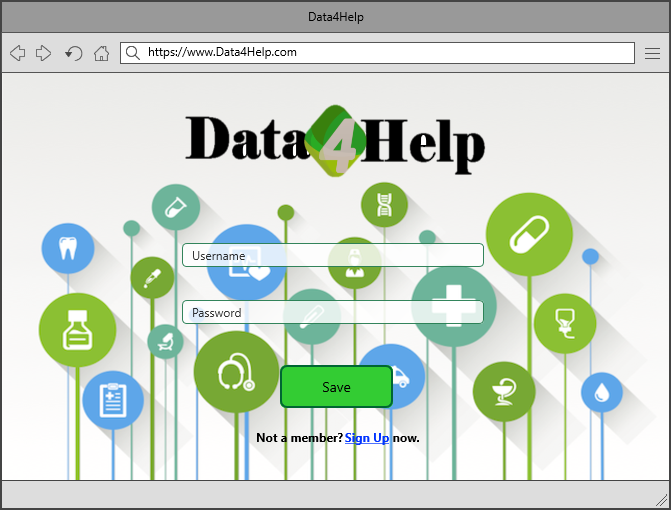
\includegraphics[width=0.795\textwidth]{./pictures/login.png}\par
	\caption{Mock up - Login}
\end{figure}
\FloatBarrier
\begin{figure}[h!]
	\centering
	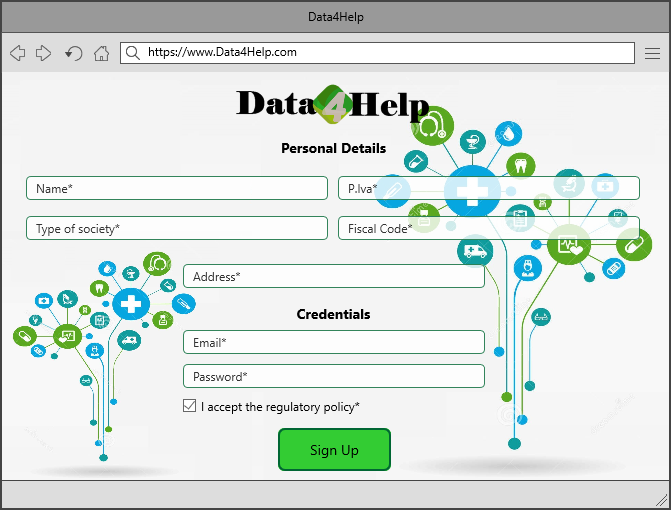
\includegraphics[width=0.795\textwidth]{./pictures/registration.png}\par
	\caption{Mock up - Registration}
\end{figure}
\FloatBarrier
\begin{figure}[h!]
	\centering
	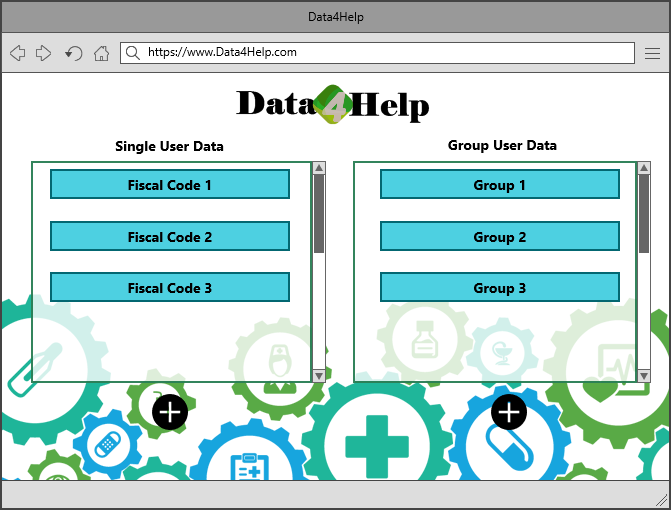
\includegraphics[width=0.80\textwidth]{./pictures/main_scene.png}\par
	\caption{Mock up - Main Scene}
\end{figure}
\FloatBarrier
\begin{figure}[h!]
	\centering
	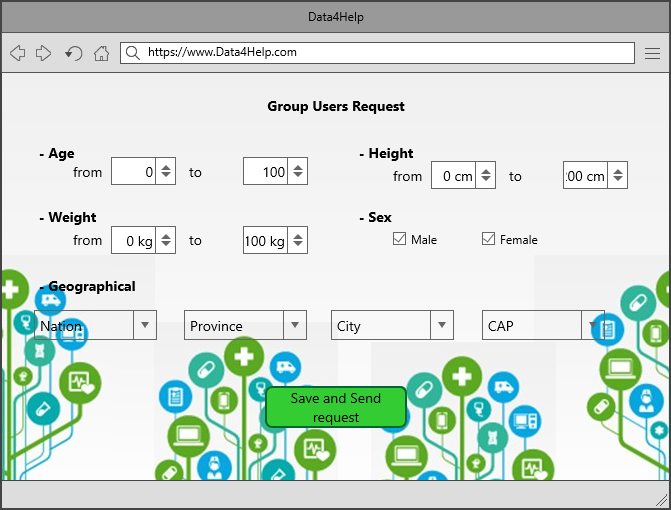
\includegraphics[width=0.80\textwidth]{./pictures/group_request.png}\par
	\caption{Mock up - Settings for a group of users request.}
\end{figure}
\FloatBarrier
\begin{figure}[h!]
	\centering
	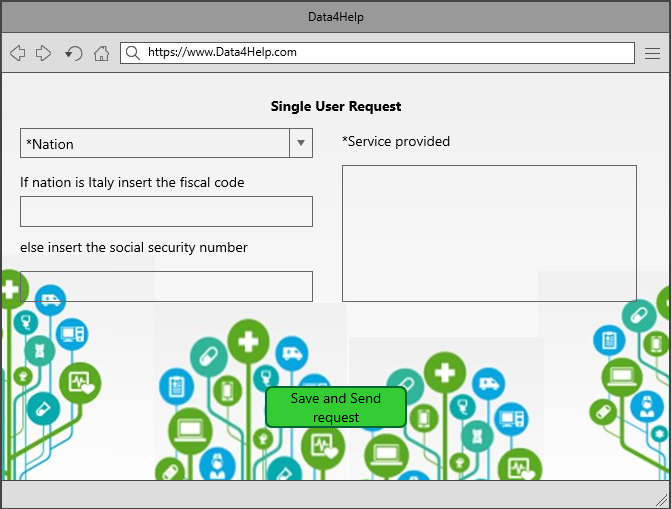
\includegraphics[width=0.80\textwidth]{./pictures/single_request.png}\par
	\caption{Mock up - Settings for a single user request.}
\end{figure}
\FloatBarrier
\begin{figure}[h!]
	\centering
	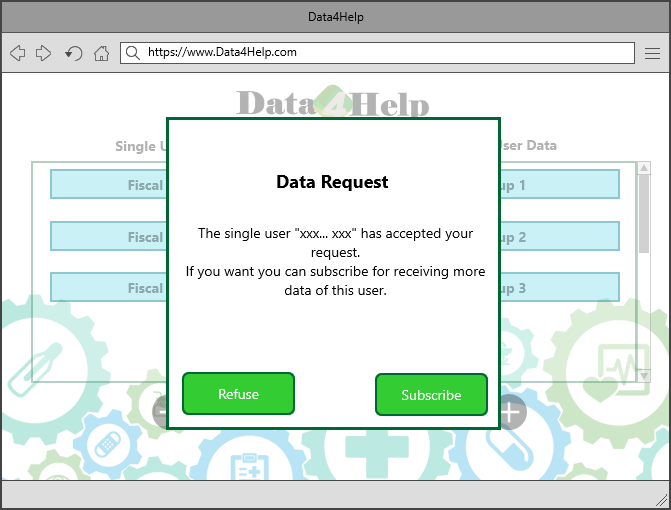
\includegraphics[width=0.80\textwidth]{./pictures/positive_request.png}\par
	\caption{Mock up - Positive notification related to a single user request. It is similar in case of a positive group of users request.}
\end{figure}
\FloatBarrier
\begin{figure}[h!]
	\centering
	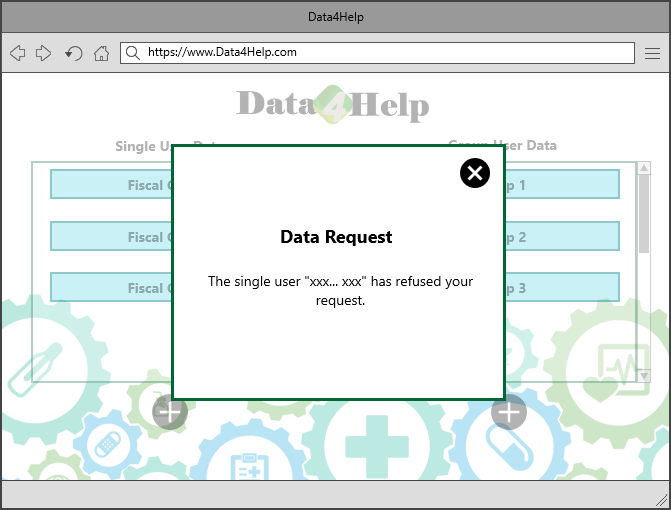
\includegraphics[width=0.80\textwidth]{./pictures/negative_request.png}\par
	\caption{Mock up - Negative notification related to a single user request. It is similar in case of a negative group of users request.}
\end{figure}
\FloatBarrier
\begin{figure}[h!]
	\centering
	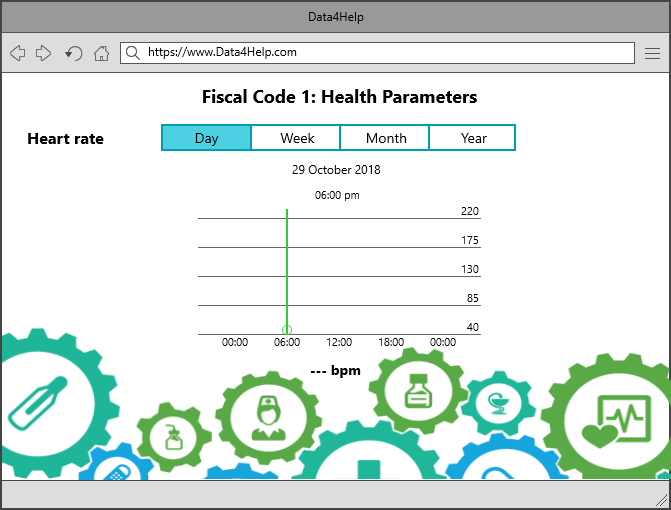
\includegraphics[width=0.80\textwidth]{./pictures/single_user_param.png}\par
	\caption{Mock up - Area realted to a fiscal code.}
\end{figure}
\FloatBarrier



	%Requirements traceability
	\chapter{Requirements Traceability}
	\label{ch: Requirements Traceability}


	%Implementation, integration and test plan
	\chapter{Impletementation, Integration and Test Plan}
	\label{ch: Impletementation, Integration and Test Plan}

	%Appendix
	\appendix
	\chapter{Appendix}
	\section{Software and tools used}
The following are all tools used to produce this document:
\begin{itemize}
	\item \textbf{\LaTeX:} used as typesetting system to build this document;
	\item \textbf{Draw:} used to draw a few diagrams such as the E-R diagram (online version can be found at \url{http://				www.draw.io});
	\item \textbf{StarUML:} used to draw some diagrams (the latest version is 3.0.2 and it can be found at \url{http://staruml.io/			download});
	\item \textbf{Mockplus:} used to draw the mockups (the latest Windows' version is 3.4.1.0 and it can be found at \url{https://			www.mockplus.com/download});
	\item \textbf{GitHub:} used to work in a distributed way and to manage different versions of the document (it can be download at		\url{https://github.com});
	\item \textbf{GitHub Desktop:} this is the official GitHub app which offers a simple and user friendly way to contribute to a git 			project (it can be download at \url{https://desktop.github.com/});
\end{itemize}

\section{Efford Spent}
The major part of the document has been produced working togheder and that's the reason way there is not a precise division of hours per sections and per group component.\\
The following is an approximate extimation of the number of hours of work for each group member:
\begin{itemize}
\item Alessandra Pasini: \textasciitilde 40 hrs;
\item Stefano Bagarin: \textasciitilde 40 hrs;
\end{itemize}

\section{Bibliography}
\begin{itemize}
	\item AA 2018/2019 Software Engineering 2 - \emph{Requirements Analysis and Specification Document} - Stefano Bagarin, 			Alessandra Pasini
	\item 2015 O'Reilly -  \emph{Software Architecture Patterns} - Mark Richards
	\item slides of \emph{Software Engineering I - II}
\end{itemize}


\end{document}


